\chapter{CÀI ĐẶT GIẢI PHÁP}

\tab Trong phần này, để cài đặt của các chức năng ở mục \ref{sec:CaiDatChucNangHeThong} "Cài đặt chức năng hệ thống" dễ hiểu và ngắn gọn hơn.
Sau khi trình bày ở mục sau xong, thì các cài đặt có liên quan tới các thư viện đó ở mục \ref{sec:CaiDatChucNangHeThong} sẽ không được miêu tả lại.

Nhóm sẽ tiến hành trình bày theo thứ tự các phần như sau:
\begin{itemize}
  \item RTK Query: cung cấp cái nhìn tổng quan về thư viện và mô tả chức năng.
  Thư viện là một trong những phần cốt lõi để cài đặt ứng dụng web.
  \item RxJS: cung cấp cái nhìn tổng quan về thư viện và mô tả chức năng tương tự cách trình bày RTK Query.
  Thư viện là một trong những phần cốt lõi để cài đặt ứng dụng hệ thống.
  \item OWASP Zed Attack Proxy: mô tả chi tiết thông tin và chức năng của ứng dụng OWASP Zed Attack Proxy.
  Làm nền tảng để tiếp trục trình bày ở mục \ref{sec:CaiDatKienTrucHeThong} "Cài đặt kiến trúc hệ thống" tiếp theo và mô tả cài đặt các chức năng ở mục \ref{sec:CaiDatChucNangHeThong} tiếp theo.
  \item Cài đặt kiến trúc hệ thống: mô tả chi tiết cách cài đặt các service đã trình bày ở phần "Thiết kế kiến trúc hệ thống tầng ứng dụng" của mục \ref{subsec:TKKienTrucHeThong}.
\end{itemize}

Việc trình bày phần này là quan trọng. Vì phần này mang các cài đặt cốt lõi của ứng dụng hệ thống, 
nếu không được mô tả trước thì sẽ khó để mô tả cài đặt các chức năng ở mục \ref{sec:CaiDatChucNangHeThong} "Cài đặt chức năng hệ thống" tiếp theo.

\section{RKT Query} \label{sec:RTKQ}

\tab Nhóm sử dụng thư viện React, là một thư viện JavaScript giúp xây dựng giao diện người dùng, để phát triển ứng dụng web.
Khi sử dụng React thì việc quản lý trạng thái ứng dụng (state) là một trong những vấn đề tiên quyết cần giải quyết.
Nhóm chọn sử dụng thư viện Redux để giải quyết vấn đề này.
Redux là một thư viện JavaScript, dùng để quản lý state ứng dụng, được sử dụng rộng rãi trong hệ sinh thái React.
\par

Trong quá khứ, trước phiên bản React 16.8, để có thể theo dõi trạng thái và vòng đời của một thành phần React (React component) thì sử dụng thành phần lớp React (React class component) là cách duy nhất.
Khi đó, việc sử dụng Redux trong ứng dụng React có đôi chút khó khăn và dài dòng do cú pháp, cấu trúc phức tạp.
Từ phiên bản React 16.8, với sự xuất hiện của thành phần hàm React (React functional component) là cách khởi tạo React component mới, cùng với sự xuất hiện của React Hook là cách quản lý trạng thái và vòng đời của component trong React functional component, thì Redux cũng được cải tiến để phù hợp với sự thay đổi này đó là sự xuất hiện của thư viện Redux Tookit.
Do đó, đề xuất sử dụng Redux của nhóm chính là sử dụng Redux Tookit.
\par

\textit{"Redux Toolkit là phương pháp tiêu chuẩn chính thức để viết logic Redux.
  Nó bao bọc xung quanh lõi của Redux, và chứa các gói và hàm được cho là cần thiết để xây dựng một ứng dụng Redux.
  Redux Toolkit tích hợp các thực hành tốt nhất (best practices) được đề xuất, đơn giản hóa hầu hết các tác vụ Redux, ngăn ngừa những sai lầm phổ biến và làm cho việc viết ứng dụng Redux dễ dàng hơn."} \cite{chap4bib1}
\par

Trong phạm vi khóa luận, khi xây dựng ứng dụng web thì việc tương tác và quản lý dữ liệu API cũng là một vấn đề tiên quyết.
Khi muốn đưa dữ liệu từ API lên trạng thái toàn ứng dụng (global state) thì ta chuyển dữ liệu này lên Redux store (đối tượng quản lý global state của Redux).
Redux là một thư viện đồng bộ và tác vụ tương tác với API là tác vụ bất đồng bộ nên thực hiện việc này sẽ có khó khăn, mã dài dòng và khó quản lý lỗi.
Để giải quyết vấn đề này, Redux Tookit có cung cấp hàm createAsyncThunk giúp đơn giản hóa quá trình tạo ra tác vụ bất đồng bộ.
Tuy nhiên, người dùng vẫn phải viết một số lượng logic đáng kể để quản lý dữ liệu ghi đệm và trạng thái tải.
Nhóm đề xuất sử dụng Redux Toolkit Query (RTK Query) làm công cụ tương tác, quản lý dữ liệu khi tương tác với API cho ứng dụng.
\par

\textit{“RTK Query là một công cụ lấy dữ liệu (fetching) và lưu đệm (caching) mạnh mẽ.
  Nó được thiết kế để đơn giản hóa các trường hợp phổ biến khi tải dữ liệu trong một ứng dụng web, loại bỏ nhu cầu viết thủ công các logic lấy dữ liệu và caching của bạn.}
\par

\textit{RTK Query là một addon tùy chọn được bao gồm trong gói Redux Toolkit, và chức năng của nó được xây dựng trên các API khác trong Redux Toolkit.“} \cite{chap4bib2}
\par

Dữ liệu và trạng thái của API được tạo với RTK Query được lưu trữ và quản lý trên store của Redux.
Thiết kế của RTK Query được lấy cảm hứng từ các công cụ phổ biến, tiên phong trong giải pháp lấy dữ liệu API như Apollo Client, React Query, Urql và SWR.
Vậy nên việc sử dụng RTK Query là giải pháp cho tương tác API kết hợp với Redux Tookit trong ứng dụng sẽ giúp cho việc quản lý trạng thái ứng dụng và tương tác với API trở nên đơn giản, dễ dàng và hiệu quả hơn.

\subsubsection{Endpoints, Queries, Mutations, các lifecycle hook và Streaming Update}

\tab Việc tương tác với API trong RTK Query xoay quanh việc cài đặt các endpoint.
Endpoint trong RTK Query được định nghĩa trong hàm createApi của thư viện.
Để định nghĩa một endpoint, chúng ta cần cung cấp các thông tin như tên endpoint (là duy nhất trong phạm vi của hàm createAPI) , địa chỉ URL của API, phương thức của endpoint (phương thức HTTP, thông tin này là tùy chọn, mặc định sẽ tùy theo loại endpoint mà ta sử dụng).
Có thể sử dụng các endpoint đã được định nghĩa trong các component của ứng dụng bằng cách sử dụng hook tương ứng.
Các hook này được sinh ra tự động bởi RTK Query và có tên được đặt dựa trên tên của endpoint.
Ví dụ, nếu endpoint được định nghĩa theo loại Query endpoint và có tên là "getUsers", thì hook để sử dụng endpoint này sẽ có tên là "useGetUsersQuery".
Ngoài ra, cũng có thể sử dụng các endpoint  qua đối tượng trả về của hàm createApi, không qua hook.
Có hai loại endpoint trong RTK Query là Query endpoint và Mutation endpoint.

\begin{itemize}
  \item \textbf{Query endpoint} khuyến cáo nên được sử dụng khi lấy, truy xuất dữ liệu từ API.
        Khi sử dụng endpoint này, theo mặc định, query endpoint sẽ tự động thực thi khi component sử dụng nó được hiển thị.
        RTK Query sẽ kiểm tra xem dữ liệu đã được lưu trong store hay chưa.
        Nếu có, dữ liệu đã có trong bộ đệm sẽ được trả về mà không cần gửi yêu cầu đến server.
        Nếu chưa có, yêu cầu sẽ được gửi đến server để lấy dữ liệu mới nhất.
  \item \textbf{Mutation endpoint} khuyến cáo nên được sử dụng khi thay đổi dữ liệu, làm cũ dữ liệu trong store qua API.
        Không như query endpoint, mutation endpoint không được thực hiện tự động mà phải gọi tới mỗi khi sử dụng.
        Endpoint này có thể sử dụng để đánh dấu dữ liệu đã cũ trong store, ra hiệu cho các endpoint có liên quan làm mới lại dữ liệu, ví dụ như component có sử dụng Query endpoint sẽ lấy dữ liệu mới, loại bỏ dữ liệu đã cũ trong store.
\end{itemize}

Endpoint của RTK Query có cung cấp nhiều lifecycle hook mạnh mẽ, hỗ trợ rất nhiều trong việc đóng gói các logic đi kèm bên trong chính endpoint đó.
Các lifecycle hook tiêu biểu được cung cấp trong cả Query endpoint và Mutation endpoint là transformResponse,  transformErrorResponse, onQueryStarted và onCacheEntryAdded.
Đặc biệt, trong Query endpoint có cung cấp hook providesTags và trong Mutation endpoint có cung cấp hook invalidatesTags.
Chi tiết của các hook này như sau:

\begin{itemize}
  \item \textbf{transformResponse:} dùng để cài đặt thay đổi, biến đổi dữ liệu (data) được trả về.
        Dữ liệu được trả về phải đi qua hook này trước khi được lấy ra từ endpoint
  \item \textbf{transformErrorResponse:} tương tự như transformResponse nhưng dành cho đối tượng lỗi (error).
  \item \textbf{onQueryStarted:} đây là một hook bất đồng bộ, các cài đặt trong hook này sẽ được thực hiện trước khi request của endpoint được gửi đi. Hook này có cung cấp đối tượng LifecycleApi chứa các phương thức để tương tác với dữ liệu, tham số từ endpoint.
  \item \textbf{onCacheEntryAdded:} đây cũng là một hook bất đồng bộ, các cài đặt trong hook sẽ được thực hiện khi có một mục đệm (cache entry) được thêm vào.
        Cache entry là một bộ dữ liệu của một endpoint với tham số truyền vào query đó.
        Như đã nói, RTK Query cache dữ liệu của endpoint để tối ưu số lần request, nên nếu có hai nơi gọi đến cùng một bộ endpoint và tham số thì dữ liệu sẽ được chia sẻ cho nhau.
        Vì vậy, lần đầu tiên bộ endpoint và tham số được gọi là lần cache entry được thêm vào.
        Hook này có cũng cấp đối tượng CacheLifecycleApi có tác dụng tương tự với LifecycleApi từ onQueryStarted.
        CacheLifecycleApi còn có cung cấp thêm hai thuộc tính là cacheDataLoaded và cacheDataRemoved để hỗ trợ ta có thể cài đặt đồng bộ trong hook.
  \item \textbf{providesTags:} Hook chỉ tồn tại trong Query endpoint.
        Hook giúp cho các Query endpoint tự động làm mới dựa trên các thẻ (tag) mà ta gắn vào.
  \item \textbf{invalidatesTags:} Hook chỉ tồn tại trong Mutation endpoint.
        Hook giúp xác định cache data nào sẽ được tìm nạp lại hoặc xóa khỏi store.
        Khi Mutation endpoint có gắn tag được gọi, dữ liệu nằm trong Query endpoint có tag tương tự sẽ bị đánh dấu là đã cũ.
        Nếu Query endpoint có dữ liệu đã bị đánh dấu cũ thì endpoint đó sẽ được thực hiện gọi lại để làm mới dữ liệu.
\end{itemize}

Trong onQueryStarted và onCacheEntryAdded của Query endpoint, hai đối tượng LifecycleApi và CacheLifecycleApi đều có cung cấp thêm thuộc tính updateCachedData.
updateCachedData hoạt động như một hàm hỗ trợ việc cập nhật dữ liệu lên đối tượng data của endpoint.
updateCachedData thay đổi dữ liệu giống với cách reducer của Redux.
\par

Có thể điều chỉnh cấu hình endpoint trong cài đặt hay trên hook để thay đổi hành vi của các endpoint.
Một trong những hành vi tiêu biểu nhóm cần trong phạm vi thực hiện khóa luận là cập nhật dữ liệu liên tục (streaming update).
Ta khởi tạo kết nối socket hay event source trong hook onCachedEntryAdded, phối hợp với sử dụng cacheDataLoaded và cacheDataRemoved để thực hiện hành vi này, chi tiết như đoạn trích ở dưới.
\par

\textit{“… bạn sẽ await cacheDataLoaded để xác định thời điểm dữ liệu đầu tiên được tải xuống, sau đó sử dụng tiện ích (utility) updateCacheData để áp dụng các streaming updates khi nhận được tin nhắn (messages).
  updateCacheData là một callback do Immer cung cấp, nhận bản draft của giá trị cache hiện tại.
  Bạn có thể biến đổi giá trị draft để cập nhật giá trị đó khi cần dựa trên các giá trị nhận được.
  RTK Query sau đó sẽ gửi một hành động áp dụng một bản vá lỗi khác dựa trên những thay đổi đó."} \cite{chap4bib3}

\section{RxJS và Reactive Programming}

\subsection{Reactive Programming}

\tab Reactive programming là thuật ngữ chỉ phương pháp xử lý, lập trình với dữ liệu không tuần tự.
Dữ liệu trong reactive programming sẽ được chứa trong một dòng tuần tự (stream) tương tự như hình \ref{fig:StreamInRP}.

\begin{figure}[H]
  \centering
  \includegraphics[width=\textwidth]{applied-thesis-chapters/chapter-4/Minh họa Stream trong Reactive Programming.png}
  \caption{Minh họa Stream trong Reactive Programming \cite{chap4bib4}}
  \label{fig:StreamInRP}
\end{figure}

Khi stream nhận vào một gói dữ liệu mới, gói đó sẽ được stream vận chuyển đến các điểm chỉnh sửa (modifier).
Modifier là các phương thức được cài đặt, có nhiệm vụ sẽ tự động chạy hay phản ứng (react) với các gói dữ liệu được đưa vào, chỉnh sửa và đưa lại về stream.
\par

Modifier tự động phản ứng với các gói dữ liệu được stream truyền vào, không cần phải tự gọi các modifier như các logic bình thường nên luồng hoạt động của mô hình này dễ đọc hiểu và nắm bắt.
Trong mô hình này, ta có thể tự định nghĩa thứ tự, logic của các modifier trong stream lúc cài đặt.
Tùy vào thứ tự, cách cài đặt của modifier mà các gói dữ liệu trong stream sẽ được thay đổi khác nhau.

\subsection{RxJS}

\tab RxJS, tên đầy đủ nhưng hiếm khi được gọi là ReactX JS, là một thư viện JavaScript dùng để xử lý event được dùng rất rộng rãi hiện nay.
Thư viện được xây dựng dựa trên khái niệm Reactive Programming, cung cấp một cách tiếp cận đơn giản và mạnh mẽ để xử lý các luồng dữ liệu.
Nó có thể sử dụng JavaScript, không phân biệt ứng dụng web hoặc ứng dụng máy chủ.
\par

\textit{“RxJS kết hợp mẫu Observer (Observer pattern) với mẫu Iterator (Iterator pattern) và lập trình hàm (functional programing) với các bộ sưu tập (collections) để quản lý các chuỗi sự kiện một cách lý tưởng.”} \cite{chap4bib5}
\par

Các khái niệm thiết yếu trong RxJS là: \cite{chap4bib5}

\begin{itemize}
  \item \textbf{Observable:} là một đối tượng đại diện cho một chuỗi các sự kiện hoặc giá trị được phát ra theo thời gian.  Có thể hiểu đây là một stream trong Reactive Programming.
  \item \textbf{Observer:} là một tập hợp các callback lắng nghe các giá trị do Observable cung cấp.
        Có ba loại callback trong đối tượng này, mỗi loại callback sẽ có chức năng khác nhau:
        \begin{itemize}
          \item next: callback này sẽ phản ứng mỗi khi Observable của nó phát ra gói dữ liệu.
          \item error: callback này sẽ phản ứng khi luồng logic trong Observable của nó phát ra lỗi, tham số trả về trong callback sẽ là lỗi mà Observable gặp phải.
          \item complete: callback này sẽ phản ứng khi logic của Observable của nó hoàn thành, không còn gói dữ liệu mới phát ra nữa.
        \end{itemize}
  \item \textbf{Subscription:} là đối tượng đại diện cho quá trình đăng ký (subscribe) và hủy đăng ký (unsubscribe) của các Observer với một Observable.
        Là cách tiếp cận tốt để quản lý các đăng ký và giải phóng tài nguyên.
  \item \textbf{Operators:} là các hàm được sử dụng để thực hiện các thao tác trên các Observable, có thể hiểu đây là các Modifier trên stream.
        Các Operators cho phép ta xử lý các logic phức tạp trong Observable đơn giản, hiệu quả và tiện lợi.
        Các Operators có thể được chia thành hai loại chính: Operators nối tiếp (Pipeable Operators) và Operators khởi tạo (Creation Operators).
        \begin{itemize}
          \item \textbf{Pipeable Operators:} sử dụng để thực hiện các thao tác trên Observable.
                Có thể sử dụng phương thức pipe() kết nối các operator với nhau, tạo ra một chuỗi các operator.
                Pipeable Operators bao gồm map(), filter(), mergeMap() và nhiều hàm khác.
          \item \textbf{Creation Operators:} sử dụng để tạo ra một Observable mới.
                Creation Operators bao gồm of(), from(), interval() và nhiều hàm khác.
        \end{itemize}
  \item \textbf{Subject:} là một loại Observable, tương đương với một EventEmitter, có thể được sử dụng trực tiếp để phát ra các sự kiện hoặc giá trị cho nhiều Observers.
  \item \textbf{Schedulers:} là các bộ điều phối tập trung để kiểm soát các hoạt động đồng thời, có thể hiểu đơn giản là sử dụng để kiểm soát và quản lý các hoạt động thực thi theo thứ tự mong muốn.
        Ngoài ra, có thể sử dụng để xác định các nguồn thực thi, thời điểm thực thi trong các Observable, cho các hoạt động đồng bộ và không đồng bộ.
        Schedulers cung cấp các tính năng như điều khiển tốc độ thực thi các hoạt động, điều chỉnh thời gian đợi giữa các hoạt động, phân tán hoạt động cho các luồng thực thi khác.
        Schedulers được đóng gói thành các loại khác nhau gồm:
        \begin{itemize}
          \item asapScheduler: dùng để kiểm soát các hoạt động đồng bộ, ưu tiên thực hiện các hoạt động ngay khi có thể.
          \item queueScheduler: dùng để kiểm soát các hoạt động đồng bộ và không đồng bộ, đưa các hoạt động vào một hàng đợi và thực hiện chúng theo thứ tự.
          \item asyncScheduler: dùng để kiểm soát các hoạt động không đồng bộ, chạy các hoạt động trong một luồng thực thi riêng biệt.
        \end{itemize}
\end{itemize}

\section{OWASP Zed Attack Proxy}

\subsection{Giới thiệu tổng quan}

\tab OWASP Zed Attack Proxy (ZAP) là một công cụ kiểm thử bảo mật ứng dụng web mã nguồn mở được phát triển bởi một cộng đồng quốc tế có tên Open Web Application Security Project (OWASP).
\par

OWASP được điều hành bởi một tổ chức có tên The OWASP Foundation tại Hoa Kỳ, được thành lập vào năm 2001 và trở thành một tổ chức từ thiện phi lợi nhuận vào ngày 21 tháng 4 năm 2004.
Tổ chức hoạt động với những giá trị cốt lõi là minh bạch, sáng tạo, toàn cầu hóa và trung thực.
Mục đích và tầm nhìn của The OWASP Foundation là loại trừ các phần mềm không an toàn.
Đến hiện tại, tổ chức đã có hơn 400 chi nhánh trên khắp thế giới, cụ thể là 448 chi nhánh vào 11/2022 . OWASP đã và đang thực hiện hơn 270 dự án, cụ thể là 276 dự án vào 11/2022. Và OWASP ZAP là một trong những dự án đó.
\par

Công cụ ZAP được sử dụng để tìm kiếm các lỗ hổng bảo mật trong ứng dụng web bằng cách mô phỏng các cuộc tấn công và kiểm tra các yếu tố bảo mật như xác thực, truy cập, mã hóa và xử lý dữ liệu.
Đồng thời, công cụ cũng cung cấp giao diện đồ họa, cho phép người dùng kiểm tra ứng dụng web bằng cách sử dụng các kịch bản kiểm thử bảo mật đã tích hợp sẵn hoặc tự tạo.
Các kịch bản này là các loại tấn công phổ biến như SQL Injection, Cross-Site Scripting (XSS), và các cuộc tấn công khác.

\subsection{Giới thiệu chức năng} \label{subsec:IntroFunc}

\tab Trong thời điểm hiện tại, công cụ ZAP có cung cấp 28 chức năng, tiện ích là Active Scan, Add-ons, Alerts, Anti CSRF Tokens, API, Authentication, Authentication Methods, Authentication Verification Strategies, Breakpoints, Contexts, Data Driven Content, HTTP Sessions, Manipulator-in-the-middle Proxy, Marketplace, Modes, Notes, Passive Scan, Scan Policy, Scope, Scripts, Session Management, Sites Tree, Spider, Statistics, Structural Modifiers, Structural Parameters, Tags, Users.
Trong đó, có 9 chức năng cốt lõi là:

\begin{itemize}
  \item \textbf{API:} công cụ có cung cấp một hệ thống API cho phép tương tác với ZAP.
        Chức năng cho phép phát triển tích hợp ZAP vào quy trình phát triển phần mềm hay chính các phần mềm khác, và thực hiện các kiểm thử bảo mật tự động.
        Chức năng cung cấp nhiều API để tương tác với nhiều chức năng khác nhau trong ZAP, tiêu biểu là quét tự động, quản lý phiên quét, kiểm soát truy cập, và quản lý cấu hình.
        \par
        Theo mặc định, chỉ máy chủ ZAP đang chạy thì mới có thể truy cập vào API.
        Để xem thông tin chi tiết về hướng dẫn và sử dụng của chức năng này, ta truy cập giao diện web qua URL http://zap/ khi đang dùng ZAP như proxy.
        Hoặc thông qua URL http://localhost:8080/ khi ứng dụng ZAP đang chạy và máy chủ của chức năng có hoạt động, mỗi instance ứng dụng ZAP sẽ có một máy chủ khác nhau, phát trên các cổng khác nhau và dữ liệu của API trả về tương ứng với mỗi instance đó.
        Dữ liệu API được cung cấp dưới dạng các định dạng JSON, HTML và XML.
  \item \textbf{Marketplace:} tính năng này nơi chứa các thành phần mở rộng (add-on) dành cho ZAP được viết bởi các thành viện trong nhóm ZAP và cộng đồng. Các add-on này có thể được tùy chỉnh cài đặt theo nhu cầu qua giao diện ứng dụng hoặc qua chức năng API của ZAP.
  \item \textbf{Spider:} là một công cụ tự động quét toàn bộ ứng dụng web để tìm kiếm các URL và các tài nguyên trong phạm vi ứng dụng đó. Trong thời điểm hiện tại, Spider là một chức năng nằm trong các add-on của ZAP. Chức năng của Spider tương tự như AJAX Spider nhưng đảm bảo an toàn cho mục tiêu được quét, thay vào đó là kết quả quét sẽ không sâu bằng AJAX Spider.
        \par
        Khi hoạt động, Spider gửi các yêu cầu HTTP giả mạo đến trang web và thu thập các phản hồi. Sau đó phân tích các phản hồi để tiếp tục tìm kiếm các URL mới, tài nguyên, tệp JavaScript và tệp CSS. Các URL mới sẽ được thêm vào hàng đợi và quá trình quét sẽ tiếp tục cho đến khi toàn bộ ứng dụng web đã được khám phá. Thêm vào đó, Spider có cung cấp các tùy chỉnh để có thể cấu hình quá trình quét cho phù hợp với nhu cầu, có thể thực hiện qua giao diện ứng dụng hoặc qua chức năng API của ZAP.
  \item \textbf{Ajax Spider:} là một công cụ quét tự động dành riêng cho các ứng dụng web sử dụng công nghệ AJAX (Asynchronous JavaScript and XML), rất hữu ích trong việc tìm kiếm các lỗ hổng bảo mật trong các ứng dụng web động. Trong thời điểm hiện tại, AJAX Spider là một chức năng nằm trong các add-on của ZAP. Khi sử dụng, ta có thể kết hợp với Spider để có được kết quả quét tốt nhất.
        \par
        Ajax Spider hoạt động bằng cách mô phỏng các tương tác AJAX của người dùng trên trình duyệt web. Nó sẽ tìm kiếm và gửi các yêu cầu AJAX đến ứng dụng web và thu thập các phản hồi. Sau đó, nó sẽ tìm kiếm các tương tác AJAX khác và tiếp tục thực hiện quét đến khi tất cả các tương tác AJAX của ứng dụng web đã được khám phá. Hơn nữa, AJAX Spider có cung cấp các tùy chỉnh để cấu hình quá trình quét cho phù hợp với nhu cầu, có thể thực hiện qua giao diện ứng dụng hoặc qua chức năng API của ZAP.
  \item \textbf{Passive Scan:} chức năng này tự động quét một cách thụ động các gói HTTP được proxy qua ZAP. Các gói HTTP bao gồm các gói yêu cầu và các gói phản hồi. Trong quá trình quét, Passive Scan không thay đổi yêu cầu hoặc phản hồi theo bất kỳ cách nào nên việc sử dụng là an toàn cho ứng dụng được quét. Gọi Passive Scan là quét thụ động vì nó không tự quét ứng dụng web, gửi và phản hồi các gói tin được mà nó cần được bổ trợ bởi các chức năng khác trong ZAP có thể thực hiện việc này như Spider, AJAX Spider hay thực hiện thủ công trên giao diện ứng dụng ZAP. Vì vậy, nó chạy ở một luồng khác dưới nền để không ảnh hưởng đến các chức năng quét chạy trên luồng chính.
        Trong quá trình quét đến khi quét xong, thông tin các thẻ hoặc cảnh báo được tìm thấy sẽ được hiển thị lần lượt. Các tùy chọn hiển thị này được kích hoạt mặc định, nhưng cũng có thể được cấu hình. Passive Scan không đảm bảo có thể tìm thấy tất cả các lỗ hổng bảo mật có thể có trong ứng dụng web, vì nó chỉ quét những yêu cầu và phản hồi được gửi qua ZAP. Passive Scan có cung cấp các tùy chỉnh để cấu hình hành vi quét, có thể thực hiện qua giao diện ứng dụng hoặc qua chức năng API của ZAP.
  \item \textbf{Active Scan:} chức năng tự động tìm kiếm các lỗ hổng bảo mật tiềm năng bằng cách thực hiện các cuộc tấn công vào các mục tiêu đã biết trước. Các cuộc tấn công là các kỹ thuật tấn công phổ biến thường được sử dụng để kiểm tra bảo mật của ứng dụng web. Các mục tiêu được tìm thông qua phương pháp quét khám phá được cấu hình khi bắt đầu phiên quét. Các phương pháp quét dùng để khám phá các mục tiêu của Active Scan là Spider hoặc AJAX Spider.
        Thực hiện Active Scan là thực hiện tấn công vào các mục tiêu trong ứng dụng web nên có thể sẽ gây ra các tác động không mong muốn đến ứng dụng web nếu không sử dụng đúng cách. Nên lưu ý rằng Active Scan chỉ có thể tìm thấy một số loại lỗ hổng. Các lỗ hổng logic như kiểm soát truy cập bị hỏng (Broken access control), sẽ không được tìm thấy bởi bất kỳ công cụ quét lỗ hổng nào, dù là Active Scan hay tự động. Active Scan có cung cấp các tùy chỉnh để cấu hình hành vi quét, có thể thực hiện qua giao diện ứng dụng hoặc qua chức năng API của ZAP. Thêm vào đó, Active Scan có thêm phần cấu hình các quy tắc quét thông qua chức năng Scan Policies.
  \item \textbf{Fuzzer:} là một chức năng kiểm thử tự động, sử dụng kỹ thuật Fuzzing là một kỹ thuật sử dụng các gói dữ liệu (payload) không hợp lệ hoặc không mong đợi đến mục tiêu. Fuzzer hay Fuzzing là một chức năng nằm trong các add-on của ZAP. Đối với các payload sử dụng trong chức năng này, ta có thể tự tạo payload, lấy trong tập payload được xây dựng sẵn trong ZAP hay các payload được thiết kế sẵn trong add-on. Có thể tùy chỉnh thay đổi hành vi của chức năng theo mong muốn bằng các chức năng con của nó như Payload Generators, Payload Processors, Fuzz Location Processors và Message Processors. Tuy nhiên, cần phải cẩn thận khi sử dụng, vì kỹ thuật nó sử dụng là một kỹ thuật tấn công nên có thể sẽ gây ra các tác động không mong muốn cho ứng dụng web nếu không sử dụng đúng cách.
  \item \textbf{WebSockets:} là một chức năng nằm trong các add-on của ZAP có thể được sử dụng khi thực hiện kiểm thử thủ công. Sử dụng chức năng này khi kiểm thử thủ công ứng dụng web trên giao diện ứng dụng ZAP, cho phép ứng dụng ZAP can thiệp vào các kết nối WebSocket giữa máy khách và máy chủ. Các can thiệp chức năng này hỗ trợ là:
        \begin{itemize}
          \item Chặn và hiển thị gói tin trong kết nối WebSocket.
          \item Thiết lập điểm dừng (breakpoint) trên các loại gói tin cụ thể trong kết nối WebSocket.
          \item Chạy Fuzz bằng chức năng Fuzzing đã được đề cập bên trên.
          \item Passive Scan các gói tin trong kết nối WebSocket.
        \end{itemize}
\end{itemize}

\subsection{Ưu và nhược điểm}

\paragraph{Ưu điểm}
\begin{itemize}
  \item Dự án mã nguồn mở, được phát triển và hỗ trợ bởi những lập trình viên kỳ cựu và tổ chức đáng tin cậy.
  \item Cung cấp đa dạng các phương pháp kiểm thử bảo mật ứng dụng từ tự động đến thủ công.
  \item Các phương pháp kiểm thử đều có thể tùy chỉnh, cấu hình đa dạng và chi tiết.
  \item Thông tin các báo cáo đều rất chi tiết và có thể tùy chỉnh.
  \item Vì là mã nguồn mở và được phát triển bởi tổ chức phi lợi nhuận nên công cụ miễn phí cho tất cả mọi người.
\end{itemize}

\paragraph{Nhược điểm}
\begin{itemize}
  \item Giao diện người dùng đã cũ, có nhiều thông tin hiển thị tràn lan gây khó hiểu.
  \item Tài liệu hướng dẫn khó hiểu, không có đủ thông tin, phân tán khó tiếp cận.
  \item Chỉ có dạng phần mềm. Phần mềm có nhiều phiên bản dành cho nhiều mục đích, hệ điều hành khác nhau. Người dùng phải có hiểu biết, tìm hiểu một lượng thông tin nhất định mới có thể hiểu và chọn đúng phiên bản mình cần.
  \item Khó sử dụng, phức tạp đối với người dùng mới.
\end{itemize}

\section{Cài đặt kiến trúc hệ thống} \label{sec:CaiDatKienTrucHeThong}

\tab Như đã trình bày ở mục Nhóm ZAP service của mục "Thiết kế kiến trúc hệ thống tầng ứng dụng" ở phần \ref{subsec:TKKienTrucHeThong}, hệ thống bao gồm nhiều service được cài đặt tách biệt với nhau và có các tác dụng khác nhau. Trong phần này, nhóm sẽ trình bày chi tiết hơn về cách thiết kế của các service này.

\subsection{Cài đặt nhóm ZAP service} \label{subsec:CaiDatNhomZapService}

\subsubsection{Cài đặt ZAP Client service}

\tab Phần cốt lõi của service được thiết kế dựa trên gói zaproxy, gói là một nhánh nhỏ của dự án ứng dụng OWASP Zed Attack Proxy hỗ trợ ứng dụng Node.js tương tác với ứng dụng ZAP dễ dàng hơn. Để liên kết một ZAP instance, nhóm cài đặt phương thức initZapClient() làm xương sống cho service, phương thức trả về đối tượng được tạo từ lớp ZapClient trong gói zaproxy.

Để tạo mới một đối tượng với lớp ZapClient, cần cung cấp hay thuộc tính là apiKey và proxy. Giá trị apiKey là chuỗi tùy chọn, là khóa được sử dụng để xác thực khi sử dụng API với ZAP instance đó. Giá trị proxy là địa chỉ máy chủ ZAP mà ZapClient hướng tới.

Các đối tượng ZapClient sẽ được quản lý trong ZAP Client service dưới dạng cặp client id và ZapClient trong một đối tượng Map() của JavaScript. Client id là một chuỗi định danh duy nhất toàn cầu (Universally Unique Identifier, gọi tắt là UUID) được tạo ngẫu nhiên, dùng để định danh đối tượng ZapClient trong Map. Tuy nhiên, ZAP cũng có cung cấp khá nhiều API mà gói zaproxy chưa có cấu hình, hỗ trợ nên nhóm cũng tiến hành tự tạo các API còn thiếu đó, nếu cần. Nhóm thực hiện điều này thông qua phương thức requestPromise() từ lớp ZapClient với tham số là endpoint của API.

Với mỗi loại quét mà hệ thống hỗ trợ, nhóm thiết kế các phương thức như bắt đầu quét (start), dừng quét (stop), phát trạng thái quét (stream status) và lấy kết quả quét chi tiết (full result) tương ứng với loại quét đó để tương tác với phiên quét trong ZAP instance, phục vụ cho ZAP Monitor service. Do các loại quét, giải pháp khác nhau sẽ có hành vi, cách hoạt động khác nhau nên thiết kế cũng sẽ khác nhau.
\par

Đối với các phương thức start scan, mỗi loại sẽ có các cấu hình, cách thức, thiết kế khác nhau. Nói chung, các phương thức đều cần các tham số như clientId (client id, để xác định đối tượng ZapClient), url (URL hay mục tiêu quét) và config (cấu hình của phiên quét) để bắt đầu phương quét. Thông tin chi tiết về sự khác nhau của các phương thức như sau:
\par

\begin{itemize}
  \item Đối với ZAP Spider, nhóm tạo phương thức spiderStart() trong service để xử lý tác vụ này.
        Phương thức có tham số clientId được xử lý đặc biệt.
        Nếu tham số clientId được chỉ định rõ ràng thì phiên quét sẽ được start trên chính ZAP Client đó.
        Nếu tham số clientId không được chỉ định rõ ràng thì phiên quét sẽ được start trên ZAP Client Shared.
        Khi đó phương thức sẽ trả về một đối tượng có chứa thứ tự của phiên quét trong ZAP instance (gọi là scan id, tên thuộc tính là scanId).
        Nếu tham số config không được chỉ định thì phương thức sẽ sử dụng cấu hình mặc định trong ZAP instance.
        Cấu hình chi tiết cho phiên quét của ZAP Spider được mô tả trong bảng \ref{tab:ConfigSpider} ở dưới.
        
        \newpage
        \begin{tabularx}{\textwidth}{|>{\hsize=.15\hsize\centering\let\newline
          \\\arraybackslash}X|>{\hsize=.15\hsize\centering\let\newline
          \\\arraybackslash}X|>{\hsize=.50\hsize\raggedright\let\newline
          \\\arraybackslash}X|}
          \hline
          \thead{Tên tham số}
           & \thead{Giá trị \\ mặc định}
           & \thead{Mô tả}
          \\
          \hline
          maxChildren
           &
          0
           &
          Tham số sử dụng để giới hạn số lượng URL con được tìm kiếm tại mỗi nút trong cây tìm kiếm. Tham số bằng 0 thể hiện số nút tìm kiếm là không giới hạn.
          \\
          \hline
          recurse
           &
          true
           &
          Tham số chỉ định cách thức tìm kiếm liên kết. Nếu giá trị là "true", Spider sẽ tìm kiếm các liên kết trên các trang con của trang web hiện tại. Nếu giá trị là "false", Spider chỉ tìm kiếm các liên kết trên trang web hiện tại mà không tìm kiếm các trang con.
          \\
          \hline
          contextName
           &
          ““
           &
          Tham số chỉ định tên của bối cảnh (context). Context là một cấu hình bao gồm các quy tắc như bao gồm (include) hoặc loại trừ (exclude) các URL có liên quan đến URL có trong quy tắc. Các cấu được lưu sẵn với tên, gọi là contextName. Đặt giá trị contextName là tên context đã lưu sẵn để sử dụng cấu hình.
          \\
          \hline
          subtreeOnly
           &
          true
           &
          Tham số chỉ định các thức truy cập các tài nguyên nằm dưới điểm bắt đầu. Nếu giá trị là “true“, Spider sẽ chỉ tìm kiếm các liên kết và trang web con của trang web bắt đầu.
          \\
          \hline
          \caption{Cấu hình phương thức quét ZAP Spider}
          \label{tab:ConfigSpider}
        \end{tabularx}

  \item Đối với ZAP Ajax, nhóm tạo phương thức ajaxStart() trong service để xử lý tác vụ này. Mỗi phiên quét của loại quét này chỉ có thể chạy trong mỗi ZAP instance tại một thời điểm. Nên mỗi khi start phiên quét, nhóm tạo mới một ZAP instance mới và start phiên quét trên instance đó. Ngoài ra, loại quét này còn cần quyền sử dụng trình duyệt (browser) để thực hiện các cuộc tấn công. Vì vậy, nhóm thực hiện cài đặt Firefox browser trong ứng dụng hệ thống và cấu hình cho phiên quét sử dụng firefox-headless (tính năng của trình duyệt Firefox, cho phép chạy trình duyệt dưới nền) trong phương thức ajaxStart(). Nhóm còn đặt các cấu hình mặc định, không bao gồm trong tham số config, trên ZAP instance trước khi start phiên quét. Các cấu hình như sau:
        \begin{itemize}
          \item Số lượng browser chạy cùng lúc là 1, qua phương thức \\
                ajaxSpider.setOptionNumberOfBrowsers() từ ZAP Client.
          \item Độ sâu tối đa mà trình crawler có thể đạt là 5, qua phương thức \\
                ajaxSpider.setOptionMaxCrawlDepth() từ ZAP Client. Mặc định của ZAP instance là 10.
          \item Thời gian mà trình crawler có thể chạy là 5 phút, qua phương thức \\
                ajaxSpider.setOptionMaxDuration() từ ZAP Client. Mặc định của ZAP instance là 60 phút.
        \end{itemize}
        Nếu tham số config không được chỉ định thì phương thức sẽ sử dụng cấu hình mặc định trong ZAP instance

        Cấu hình chi tiết cho phiên quét của ZAP Ajax được mô tả trong bảng \ref{tab:ConfigAjax} ở dưới.

        \begin{tabularx}{\textwidth}{|>{\hsize=.15\hsize\centering\let\newline
          \\\arraybackslash}X|>{\hsize=.15\hsize\centering\let\newline
          \\\arraybackslash}X|>{\hsize=.50\hsize\raggedright\let\newline
          \\\arraybackslash}X|}
          \hline
          \thead{Tên tham số}
           & \thead{Giá trị \\ mặc định}
           & \thead{Mô tả}
          \\
          \hline
          inScope
           &
          false
           &
          Nếu tham số có giá trị là “true” thì mọi URL nằm ngoài phạm vi sẽ bị bỏ qua.
          \\
          \hline
          contextName
           &
          ““
           &
          Tham số chỉ định tên của bối cảnh hoạt động. Chi tiết giống với bảng x ở trên.
          \\
          \hline
          subtreeOnly
           &
          true
           &
          Tham số chỉ định các thức truy cập các tài nguyên nằm dưới điểm bắt đầu. Chi tiết giống với bảng x ở trên.
          \\
          \hline
          \caption{Cấu hình phương thức quét ZAP Ajax}
          \label{tab:ConfigAjax}
        \end{tabularx}
  \item Đối với ZAP Passive, nhóm tạo phương thức passiveStart() trong service để xử lý tác vụ này.
  Loại quét này được thực hiện và kết quả được quản lý trên phạm vi toàn ZAP instance nên không thể chạy song song nhiều phiên quét. Nên giống như ZAP Ajax, nhóm tạo một ZAP instance mới cho mỗi phiên quét.
  
  Như đã nhắc đến ở mục \ref*{subsec:IntroFunc}, ZAP Passive là quét thụ động và cần được bổ trợ bởi ZAP Spider hay ZAP Ajax. Vì vậy phương thức có thêm tham số exploreType. Tham số có hai giá trị là “spider“ và “ajax“, giúp cho phương thức start biết được sẽ sử dụng ZAP Spider hay ZAP Ajax để khám phá. Khi đó, cấu hình chi tiết cho phiên quét sẽ tùy theo cách khám phá mà là cấu hình chi tiết của ZAP Spider hoặc ZAP Ajax. Phương thức không có tham số config.
  \item Đối với ZAP Active, nhóm tạo phương thức activeStart() trong service để xử lý tác vụ này.
        Loại quét này được thực hiện và kết quả được quản lý trên phạm vi toàn ZAP instance nên không thể chạy song song nhiều phiên quét, giống ZAP Passive.
        Vậy nên nhóm cũng tạo ZAP instance mới cho mỗi phiên quét.
        
        Như đã nhắc đến ở mục \ref*{subsec:IntroFunc}, các mục tiêu để tấn công cần được tìm trước thông qua ZAP Spider hay ZAP Ajax nên phương thức cũng có thêm tham số exploreType và cách xử lý giống với passiveStart().
        Ngoài ra, để đảm bảo tất cả các quy tắc quét trong chức năng Scan Policy đều được áp dụng, trước khi start phiên quét, nhóm kích hoạt tất cả các quy tắc quét Scan Policy qua phương thức ascan.enableAllScanners() từ ZAP Client.
        Nếu tham số config không được chỉ định thì phương thức sẽ sử dụng cấu hình mặc định trong ZAP instance.
        Cấu hình chi tiết cho phiên quét của ZAP Active được mô tả trong bảng \ref{tab:ConfigActive} ở dưới.
        \begin{tabularx}{\textwidth}{|>{\hsize=.20\hsize\centering\let\newline
          \\\arraybackslash}X|>{\hsize=.20\hsize\centering\let\newline
          \\\arraybackslash}X|>{\hsize=.40\hsize\raggedright\let\newline
          \\\arraybackslash}X|}
          \hline
          \thead{Tên tham số}
           & \thead{Giá trị \\ mặc định}
           & \thead{Mô tả}
          \\
          \hline
          exploreType
           &
          spider
           &
          Giống với mô tả tham số exploreType được mô tả ở mục trên.
          \\
          \hline
          recurse
           &
          true
           &
          Chi tiết giống với tham số recurse ở bảng cấu hình phương thức quét ZAP Spider.
          \\
          \hline
          inScopeOnly
           &
          false
           &
          Chi tiết giống với tham số inScope ở bảng cấu hình phương thức quét ZAP Ajax.
          \\
          \hline
          scanPolicyName
           &
          ““
           &
          Tham số này cho phép người dùng chỉ định chính sách quét được sử dụng trong quá trình quét. Nếu không có chính sách quét nào được chỉ định, công cụ quét sẽ sử dụng chính sách quét mặc định.
          \\
          \hline
          method
           &
          ““
           &
          Tham số này cho phép người dùng chọn một phương thức cụ thể để thực hiện quét, ví dụ như GET hoặc POST.
          \\
          \hline
          postData
           &
          ““
           &
          Tham số này cho phép người dùng chỉ định dữ liệu đăng được sử dụng trong quá trình quét, nếu phương thức được sử dụng là POST.
          \\
          \hline
          contextId
           &
          ““
           &
          Chi tiết tương tự với tham số contextName ở bảng cấu hình phương thức quét ZAP Spider. Nhưng chỉ số thứ tự của context đó trang danh sách đã lưu.
          \\
          \hline
          \caption{Cấu hình phương thức quét ZAP Active}
          \label{tab:ConfigActive}
        \end{tabularx}
\end{itemize}
Nếu start scan thành công thì các phương thức sẽ trả về đối tượng định danh cho phiên quét, không thành công thì trả về đối tượng không xác định.

Đối với các phương thức stop scan, các loại quét được cấu hình tương tự nhau bằng cách gọi đến phương thức stopZapClient(). Phương thức thực hiện gọi đến phương thức shutdown() từ core ZAP Client để tắt ZAP instance và xóa ZAP Client ra khỏi Map lưu trữ. Phương thức stop của ZAP Spider được cấu hình khác biệt, vì ZAP Spider riêng lẻ được chạy trên ZAP Client Shared nên sẽ được gọi đến phương thức stop() của chính phiên quét đó, sử dụng tham số scan id để xác định phiên quét.
\par

Đối với các phương thức stream status, các loại quét được cấu hình tương tự nhau bằng cách tạo một Observable kiểu timer() với RxJS và gọi đến phương thức status() của phiên quét hoặc ZAP Client đó mỗi 5 giây. Kiểu trạng thái nhận lại của mỗi loại quét sẽ khác nhau về kiểu lẫn giá trị.
\par

Đối với các phương thức lấy full result, các loại quét khác nhau sẽ có cách cài đặt khác nhau, kiểu result trả về từ ZAP khác nhau và kiểu result được lưu trữ khác nhau.

\begin{itemize}
  \item Đối với ZAP Spider, nhóm sử dụng phương thức spider.fullResult() từ ZAP Client để lấy full result của phiên quét.
        Dữ liệu trả về còn thô, khó sử dụng, lưu trữ và truy xuất nên nhóm có thực hiện biến đổi lại như sau, chi tiết cách biến đổi kiểu dữ liệu được thể hiện trong hình \ref{fig:SpiderTransformData} thể hiện kiểu dữ liệu ZAP Spider full result khi mới trả về từ ZAP instance và sau khi được biến đổi.
        \begin{figure}[H]
          \centering
          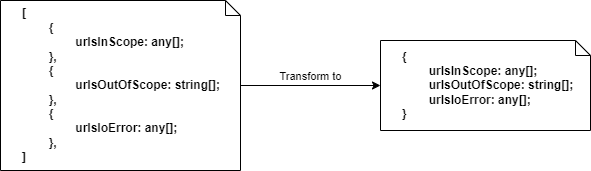
\includegraphics[width=\textwidth]{applied-thesis-chapters/chapter-4/Quá trình biến đổi của kiểu dữ liệu ZAP Spider full result.png}
          \caption{Quá trình biến đổi của kiểu dữ liệu ZAP Spider full result}
          \label{fig:SpiderTransformData}
    \end{figure}
  \item Đối với ZAP Ajax nhóm sử dụng phương thức ajaxSpider.fullResult() từ ZAP Client để lấy full result và không cần thực hiện biến đổi lại.
  \item Đối với ZAP Passive và ZAP Active, kết quả quét của hai loại này là thông tin chi tiết của các lỗ hổng tìm năng gọi là cảnh báo (alert).
  
  ZAP cung cấp khá nhiều tổ hợp thông tin này, mỗi tổ hợp có kiểu dữ liệu khác nhau.
  Nhóm chọn ra hai tổ hợp thông tin sau đó dựa vào các cách thay đổi, truy xuất tùy chỉnh để có được đầy đủ thông tin.
  Tổ hợp đầu tiên là các alert, nhóm cài đặt phương thức getClientAlerts() trong service, với tham số truyền vào là client id, để lấy danh sách tất cả các alert mà instance tìm được.
  Phương thức getClientAlerts() sử dụng phương thức core.alerts() từ ZAP Client làm xương sống.
  
  Tổ hợp tiếp theo là các alert theo rủi ro (risk), gọi là alert by risk, risk là một trường chỉ độ nghiêm trọng của alert.
  Nhóm cài đặt phương thức getClientAlertsByRisk() với tham số truyền vào là client id, hoạt động giống getClientAlerts().
  Nhóm tự tạo một API đến ZAP bằng cách sử dụng endpoint /alert/view/alertsByRisk/ với phương thức requestPromise() từ ZAP Client để hỗ trợ phương thức này.
  Tuy nhiên kết quả trả về khá khó sử dụng nên nhóm có thực hiện biến đổi lại như sau, chi tiết cách biến đổi kiểu dữ liệu được thể hiện trong hình \ref{fig:ActiveTransformData} thể hiện kiểu dữ liệu alert by risk của ZAP Active và ZAP Passive khi mới trả về từ ZAP instance và sau khi được biến đổi.
  \begin{figure}[H]
    \centering
    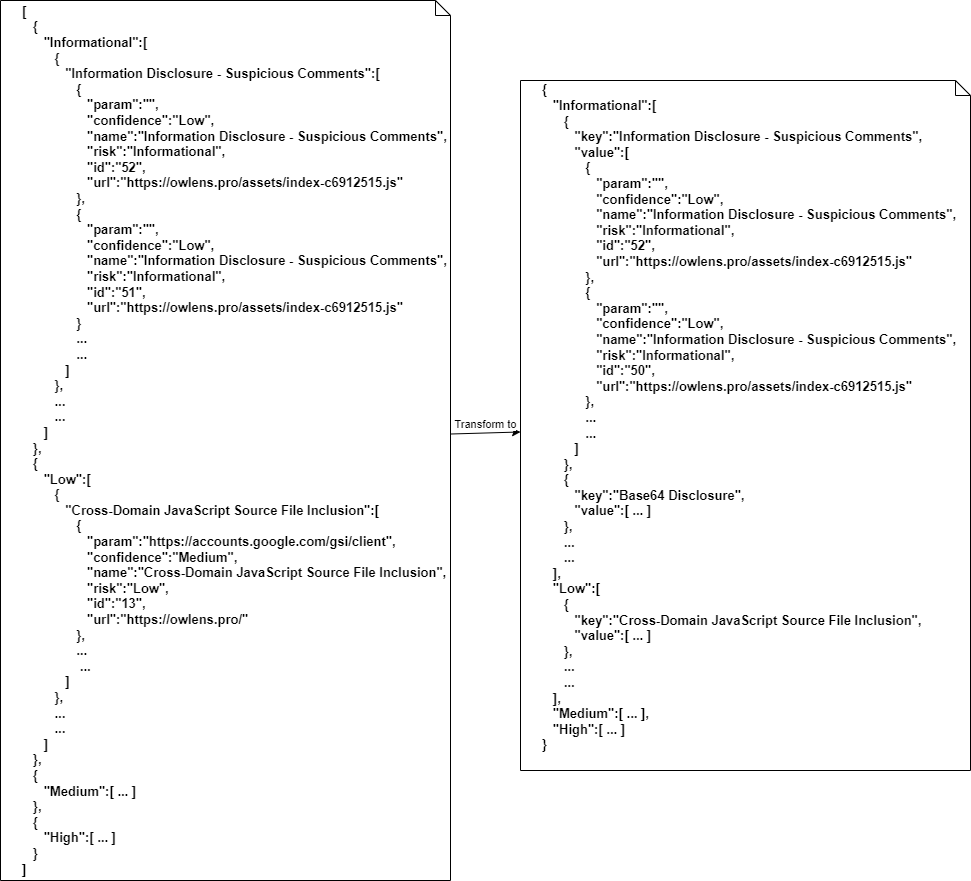
\includegraphics[width=\textwidth]{applied-thesis-chapters/chapter-4/Quá trình biến đổi của kiểu dữ liệu ZAP Active và ZAP Passive full result.png}
    \caption{Quá trình biến đổi của kiểu dữ liệu ZAP Active và ZAP Passive full result}
    \label{fig:ActiveTransformData}
\end{figure}
\end{itemize}

\subsubsection{Cài đặt ZAP Monitor service}

\tab Như đã trình bày ở mục Nhóm ZAP service của mục Thiết kế kiến trúc hệ thống tầng ứng dụng ở phần \ref{subsec:TKKienTrucHeThong}, service đóng vai trò trung gian giữa ứng dụng hệ thống và ZAP Client service.

Hệ thống thực hiện tương tác với phiên quét thông qua ZAP Monitor service.
Các tương tác với phiên quét, giống nhau với mọi loại quét, được nhóm thiết kế trong service này là start và giám sát; chia sẻ trạng thái trực tiếp; ra hiệu dừng quét.
Các phiên quét được quản lý trong service dưới dạng cặp định danh giám sát (monitor id) và đối tượng giám sát phiên quét trong một đối tượng Map() của JavaScript.
Cách thức cài đặt cho các tương tác như sau:

\begin{itemize}
  \item Với tương tác start và giám sát, các loại quét đều có thiết kế, luồng hoạt động tương tự nhau nhưng không giống nhau.
  Nhóm cài đặt các phương thức có tên với tiền tố là tên loại quét và hậu tố là StartAndMonitor để thực hiện tác vụ này, ví dụ ajaxStartAndMonitor(), nhóm sẽ gọi ngắn gọn là StartAndMonitor.
  
  Luồng hoạt động chung của các StartAndMonitor gồm các bước tuần tự là start phiên quét; tạo đối tượng giám sát phiên quét và thêm đối tượng đó vào Map giám sát.
  Monitor id là băm (hash) của đối tượng chứa client id và scan id nên đảm bảo được tính độc nhất.
  Đối tượng giám sát phiên quét, gọi là status monitor (là connectable() trong RxJS).
  Đối tượng dù để cho phép nhiều kết nối có thể đăng ký (subscribe) vào.
  Status monitor gói stream status observable của phiên quét ở bên trong (stream status observable đã nhắc đến ở mục "Cài đặt ZAP Client service" phần \ref{subsec:CaiDatNhomZapService}).
  
  Status monitor dùng để giám sát, thực hiện các tác vụ khi phiên quét đạt tới status cần xử lý và là observable được đẩy lên làm publisher (hay gọi là đối tượng phát trạng thái, emmiter).
  Các tác vụ tiêu biểu được thực hiện trong status monitor là:
  \begin{itemize}
    \item Chỉ phát status khi có thay đổi so với phiên trước (mặc định).
    \item Lấy full result của phiên quét tương ứng từ ZAP Client service và lưu xuống database qua Database service.
    \item Thực hiện giải phóng các tài nguyên liên quan trong quá trình quét như xóa status monitor khỏi Map giám sát, tắt phiên quét, tắt ZAP instance qua ZAP Client service.
  \end{itemize}
  
  \item Tương tác chia sẻ trạng thái trực tiếp, đặt tên tương tự StartAndMonitor là SharedStatusStream, dành cho ứng dụng hệ thống đưa status monitor lên làm publisher.
  Publisher gửi status phiên quét cho subscriber từ ứng dụng web bằng SSE, như thiết kế ở hình \ref{fig:TTZapMonitorStartScan} của mục "Thiết kế kiến trúc hệ thống tầng ứng dụng phần" \ref{subsec:TKKienTrucHeThong}.
  \item Tương tác ra hiệu dừng quét là phương thức thiết kế hỗ trợ cho những trường hợp đặc biệt, được sử dụng như một phương pháp thu gom thủ công trên hệ thống. Những trường hợp này là khi có lỗi không xác định xảy ra, thiết kế dành cho trường hợp đặc biệt. Đảm bảo không có phiên quét dư thừa, ảnh hưởng hiệu suất hệ thống.
\end{itemize}

\subsection{Cài đặt Authentication service}

\tab Nhóm sử dụng nền tảng bên thứ ba là Google Cloud Identity (GCI), một nền tảng quản lý truy cập và nhận diện người dùng, làm chủ chốt để cài đặt service này.
Cụ thể là sử dụng chức năng Xác thực (Authentication) trong nhóm các chức năng “Sign In with Google for Web“ của nền tảng.
Để có thể sử dụng chức năng từ nền tảng, nhóm phải tạo một Google API ID (Google API client ID) để sử dụng trên cả ứng dụng web và ứng dụng hệ thống.
Cài đặt chi tiết liên quan đến client ID này ở phía ứng dụng web sẽ được trình bày ở mục "Cài đặt chức năng đăng ký / đăng nhập phần" \ref{subsec:CaiDatDangKyDangNhap}.
\par

Ở ứng dụng hệ thống, để tương tác được với GCI, nhóm cài đặt gói google-auth-library và sử dụng đối tượng tạo từ lớp OAuth2Client với client ID đã có. Ta sử dụng đối tượng này để kiểm tra lại token credential nằm trong cookie với phương thức verifyIdToken() từ đối tượng, cookie được ghi và gửi kèm đến từ ứng dụng web. Nếu kết quả kiểm tra là hợp lệ, ta sẽ nhận được một đối tượng chứa thông tin chi tiết của tài khoản người dùng từ GCI trả về, nhóm gọi là GgUserData.
\par

Ngoài sử dụng để xác minh token credential, service được cài đặt và sử dụng chủ yếu làm các middleware ở những API có cần xác thực người dùng. Các middleware này phối hợp tuần tự với nhau, thực hiện các công việc riêng biệt để bảo vệ API nằm dưới nó. Hai middleware đầu tiên là parseAccessTokenMdw() và parseRefreshTokenMdw(), sử dụng phương thức expressjwt từ gói express-jwt, dùng để tách và xác minh lại accessToken và refreshToken, ngoài ra còn giúp các API nằm dưới truy cập token đã tách dễ hơn. Tiếp đó là middleware authenAccessMdw() dùng để kiểm tra tồn tại hợp lệ của accessToken và refreshToken đã tách, thực hiện tạo mới accessToken cho người dùng nếu accessToken đã hết hạn.
\par

Hai token trên là hai JWT được tạo qua phương thức signJwt() trong service, phương thức được cài đặt bằng cách sử dụng gói jsonwebtoken và khóa riêng tư (private key) của ứng dụng hệ thống là ZAP\_OP\_PRIVATE\_KEY.

\subsection{Cài đặt Database service}

\tab Để service kết nối và tương tác với cơ sở dữ liệu, nhóm sử dụng gói mongoose, một thư viện hỗ trợ tương tác với cơ sở dữ liệu MongoDB dành cho Node.js, để tạo kết nối với MongoDB từ MongoDB Atlas thông qua phương thức connect() được gói cung cấp và chuỗi kết nối đến cơ sở dữ liệu.
\par

Trong MongoDB, một bảng trong database gọi là Collection. Collection được đặt tên theo quy ước của MongoDB và lưu trữ các bản ghi (document) trong đó. Để tương tác với các Collection, ta cần có các đối tượng Model, mỗi Model là đại diện cho mỗi Collection trong Mongoose. Model giúp việc tương tác với MongoDB dễ dàng hơn, không cần viết các câu lệnh trực tiếp để thao tác trên cơ sở dữ liệu. Thay vào đó, ta sử dụng các phương thức có sẵn trong Model để thực hiện các thao tác tương ứng. Đồng thời, định nghĩa cấu trúc (Schema) của Collection cũng có thể được tạo trong lúc tạo Model. Để tạo các Model, ta sử dụng đối tượng đã kết nối với database và phương thức model() được cung cấp bởi thư viện mongoose.
\par

Hệ thống có bốn Model chính dành để lưu trữ dữ liệu cho target, người dùng (user), phiên quét (scan session) và kết quả quét chi tiết (scan full result). Để khởi tạo và định nghĩa các Model này, hệ thống tạo các model có tên tương ứng lần lượt là target.model, user.model, scan-session.model và scan-fullresults.model. Các Model được tạo riêng lẻ trên các tệp khác nhau và xuất đối tượng trả về của model() để chia sẻ cho các tác vụ khác.

Vì hệ thống có nhiều loại document khác nhau trên một Collection, như Collection dành cho phiên quét cần lưu trữ bốn loại phiên quét là ZAP Spider, ZAP Ajax, ZAP Passive và ZAP Active. Nên nhóm cần cấu hình cho các Model để thực hiện tác vụ này.
\par

Mongoose cung cấp một tính năng cho phép định nghĩa các loại document khác nhau trong một Collection là Discriminator. Khi sử dụng Discriminator, có thể định nghĩa một Schema chung cho tất cả các document trong Collection, sau đó định nghĩa các Schema riêng cho các document con. Các Schema riêng này sẽ kế thừa từ Schema chung và bổ sung thêm các định nghĩa của riêng nó. Document của các Schema con sẽ được phân biệt dựa trên một trường phân loại gọi là discriminator key.
\par

Để tạo các Discriminator cho các Collection cần thiết, trên đối tượng Model của Collection đó, nhóm sử dụng phương thức discriminator() cùng một chuỗi dành để phân biệt các Schema con, chuỗi này cũng chính là discriminator key. Các đối tượng trả về từ phương thức discriminator() có thể sử dụng tương tự như đối tượng từ Model, tuy nhiên đối tượng chỉ có ảnh hưởng trên chính các document của chính nó.

\subsection{Cài đặt Logging service}

\tab Service sử dụng gói winston để cài đặt và cấu hình các luồng nhật ký.
Hệ thống có thể cụ thể tạo mới hoặc hủy các log tùy chỉnh qua các phương thức registerCustomLogger() và endCustomLogger().
Các log tùy chỉnh là các loại, đối tượng log mới.
Nằm ngoài bốn loại log chủ yếu được trình bày ở phần "Logging service" của phần "Thiết kế kiến trúc hệ thống tầng ứng dụng" mục \ref{subsec:TKKienTrucHeThong}.
Các luồng log ngoài hiển thị trên console còn được lưu trữ trong thư mục có tên logs, thư này đồng cấp với thư mục chứa ứng dụng. Các loại log khác nhau hay mỗi log tùy chỉnh sẽ được lưu trong tệp riêng biệt, với tên tệp (tên luồng log được đặt lúc tạo) và thời gian tương ứng.

\section{Cài đặt chức năng hệ thống} \label{sec:CaiDatChucNangHeThong}

\tab Để thống nhất thông tin chi tiết cho trạng thái của các endpoint, nhóm thiết kế ba bảng trạng thái \ref{tab:LoginStatus}, \ref{tab:ScanStatus} và \ref{tab:MgmtStatus} riêng cho hệ thống và sử dụng tùy theo các trường hợp khác nhau.

\begin{tabularx}{\textwidth}{|>{\hsize=.35\hsize\centering\let\newline
  \\\arraybackslash}X|>{\hsize=.60\hsize\raggedright\let\newline
  \\\arraybackslash}X|}
  \hline
  \thead{Tên đại diện}
   & \thead{Đối tượng trạng thái}
  \\
  \hline
  LOGIN\_SUCCESS
   &
  statusCode: 0
  \newlinecontenttable
  msg: "Login successfully"
  \\
  \hline
  TOKEN\_NOT\_FOUND
   &
  statusCode: -1
  \newlinecontenttable
  msg: "No token found"
  \\
  \hline
  TOKEN\_INVALID
   &
  statusCode: -2
  \newlinecontenttable
  msg: "Invalid token"
  \\
  \hline
  USER\_ADD\_FAILED
   &
  statusCode: -3
  \newlinecontenttable
  msg: "New user failed to add"
  \\
  \hline
  USER\_ALREADY\_LINKED
   &
  statusCode: -4
  \newlinecontenttable
  msg: "Google account already used with different email"
  \\
  \hline
  EMAIL\_ALREADY\_USED
   &
  statusCode: -5
  \newlinecontenttable
  msg: "Email already used"
  \\
  \hline
  \caption{Trạng thái cho việc xác thực người dùng (LOGIN\_STATUS)}
  \label{tab:LoginStatus}
\end{tabularx}

\begin{tabularx}{\textwidth}{|>{\hsize=.35\hsize\centering\let\newline
  \\\arraybackslash}X|>{\hsize=.60\hsize\raggedright\let\newline
  \\\arraybackslash}X|}
  \hline
  \thead{Tên đại diện}
   & \thead{Đối tượng trạng thái}
  \\
  \hline
  SESSION\_INITIALIZE
  \newlinecontenttable
  \_SUCCEED
   &
  statusCode: 90
  \newlinecontenttable
  msg: "Scan session initialize succeed!"
  \\
  \hline
  SESSION\_INITIALIZE\_FAIL
   &
  statusCode: -91
  \newlinecontenttable
  msg: "Scan session initialize fail!"
  \\
  \hline
  INVAVLID\_URL
   &
  statusCode: -92
  \newlinecontenttable
  msg: "Invalid URL!"
  \\
  \hline
  INVALID\_SESSION
   &
  statusCode: -93
  \newlinecontenttable
  msg: "Invalid scan session!"
  \\
  \hline
  ZAP\_INITIALIZE\_FAIL
   &
  statusCode: -94
  \newlinecontenttable
  msg: "ZAP scan initialize fail!"
  \\
  \hline
  ZAP\_INTERNAL\_ERROR
   &
  statusCode: -95
  \newlinecontenttable
  msg: "ZAP internal error!"
  \\
  \hline
  INVALID\_ID
   &
  statusCode: -96
  \newlinecontenttable
  msg: "Invalid scan id!"
  \\
  \hline
  INVALID\_RESULT\_OFFSET
   &
  statusCode: -97
  \newlinecontenttable
  msg: "Invalid scan result offset!"
  \\
  \hline
  INVALID\_ID\_OR
  \newlinecontenttable
  \_ZAP\_INTERNAL\_ERROR
   &
  statusCode: -98
  \newlinecontenttable
  msg: "Invalid scan id or ZAP internal error!"
  \\
  \hline
  \caption{Trạng thái cho quá trình quét (SCAN\_STATUS)}
  \label{tab:ScanStatus}
\end{tabularx}

\begin{tabularx}{\textwidth}{|>{\hsize=.35\hsize\centering\let\newline
  \\\arraybackslash}X|>{\hsize=.60\hsize\raggedright\let\newline
  \\\arraybackslash}X|}
  \hline
  \thead{Tên đại diện}
   & \thead{Đối tượng trạng thái}
  \\
  \hline
  TARGET\_ADDED
   &
  statusCode: 10
  \newlinecontenttable
  msg: "Target added successfully"
  \\
  \hline
  TARGET\_MOVED
  \newlinecontenttable
  \_TO\_TRASH
   &
  statusCode: 11
  \newlinecontenttable
  msg: "Target moved to trash successfully"
  \\
  \hline
  TARGET\_DELETED
   &
  statusCode: 12
  \newlinecontenttable
  msg: "Target deleted successfully"
  \\
  \hline
  TARGET\_INVAVLID\_URL
   &
  statusCode: -11
  \newlinecontenttable
  msg: "Invalid URL for target"
  \\
  \hline
  TARGET\_ADD\_FAILED
   &
  statusCode: -12
  \newlinecontenttable
  msg: "Target failed to add"
  \\
  \hline
  TARGET\_INVALID\_ID
   &
  statusCode: -13
  \newlinecontenttable
  msg: "Invalid ID for target"
  \\
  \hline
  TARGET\_FIND\_FAILED
   &
  statusCode: -14
  \newlinecontenttable
  msg: "Target failed to find"
  \\
  \hline
  TARGET\_DELETE\_FAILED
   &
  statusCode: -15
  \newlinecontenttable
  msg: "Target failed to delete"
  \\
  \hline
  TARGET\_NAME
  \newlinecontenttable
  \_DUPLICATE
   &
  statusCode: -16
  \newlinecontenttable
  msg: "Target name already exist"
  \\
  \hline
  TARGET\_GET\_FAILED
   &
  statusCode: -17
  \newlinecontenttable
  msg: "Targets cannot be found"
  \\
  \hline
  SESSION\_GET\_FAILED
   &
  statusCode: -18
  \newlinecontenttable
  msg: "Sessions cannot be found"
  \\
  \hline
  \caption{Trạng thái cho các tác vụ quản lý (MGMT\_STATUS)}
  \label{tab:MgmtStatus}
\end{tabularx}

\subsection{Cài đặt chức năng đăng ký/ đăng nhập và đăng xuất} \label{subsec:CaiDatDangKyDangNhap}

\subsubsection{Cài đặt chức năng đăng ký / đăng nhập}

\tab Nhóm sử dụng nền tảng Google Cloud Identity, một nền tảng quản lý truy cập và nhận diện người dùng, làm chủ chốt để cài đặt chức năng đăng ký/đăng nhập cho ứng dụng, cụ thể là chức năng “Sign In with Google for Web“, một trong các chức năng Xác thực (Authentication) của nền tảng. Để có thể sử dụng chức năng từ nền tảng, nhóm phải tạo một Google API ID (Google API client ID), sau nhóm sẽ gọi là Google ID.
\par

Ở ứng dụng web, để sử dụng được Google Sign-In (GSI) nhóm thêm thư viện GSI dành cho phía ứng dụng khách vào bên trong thẻ <head> của tệp HTML chứa ứng dụng, chi tiết như sau:
\par

\lstset{style=mystyle}
\begin{lstlisting}[language=HTML, caption=Thêm thư viện GSI vào ứng dụng]
  <head>
  ...
    <!-- GOOGLE PLATFORM LIBRARY IMPORT -->
    <script src="https://accounts.google.com/gsi/client" async defer></script>
  ...
  </head>
\end{lstlisting}

Vì ứng dụng web được phát triển bằng React TypeScript, nên để sử dụng thư viện một cách tiện lợi nhóm cần phải cài đặt thêm gói @types/google.accounts ở thuộc tính devDependencies trong tệp package.json.

Sau khi đã cài đặt các thư viện nền tảng, nhóm tạo AuthGoogleButton component và thực hiện hóa các chức năng gói trong component này. Component thực hiện cấu hình GSI cho ứng dụng bằng phương thức initialize() từ đối tượng window.google.accounts.id có trong thư viện. Các cấu hình là Google ID và callback là phương thức xử lý thông tin xác thực (credential, là một JSON Web Tokens - JWT) của GSI trả về. Sau đó tiến hành nhúng nút GSI vào ứng dụng bằng phương thức renderButton() từ đối tượng window.google.accounts.id.

Nhóm thiết kế một mutation endpoint với RTK Query đặt tên là login, endpoint thực hiện request với phương thức HTTP POST đến điểm /login của ứng dụng hệ thống. Endpoint nhận vào biến loại GSI credential và trả về các đối tượng trạng thái như bảng trạng thái cho việc xác thực. Đồng thời, trên hook onQueryStarted của endpoint, nhóm xử lý ghi credential vào cookie tên ggToken tại domain hiện tại. Khi người dùng thực hiện đăng nhập hoàn tất, kích hoạt login endpoint.

Để thực hiện xác thực, ứng dụng hệ thống thực hiện kiểm tra xem người dùng có phải là người dùng mới hay không.
Nếu người dùng là người dùng mới thì thực hiện đăng ký cùng với đăng nhập, nếu không thì thực hiện đăng nhập.
Chi tiết trong hình \ref{fig:SignUpIn} sơ đồ luồng kiểm tra đăng nhập.

\begin{figure}[H]
  \centering
  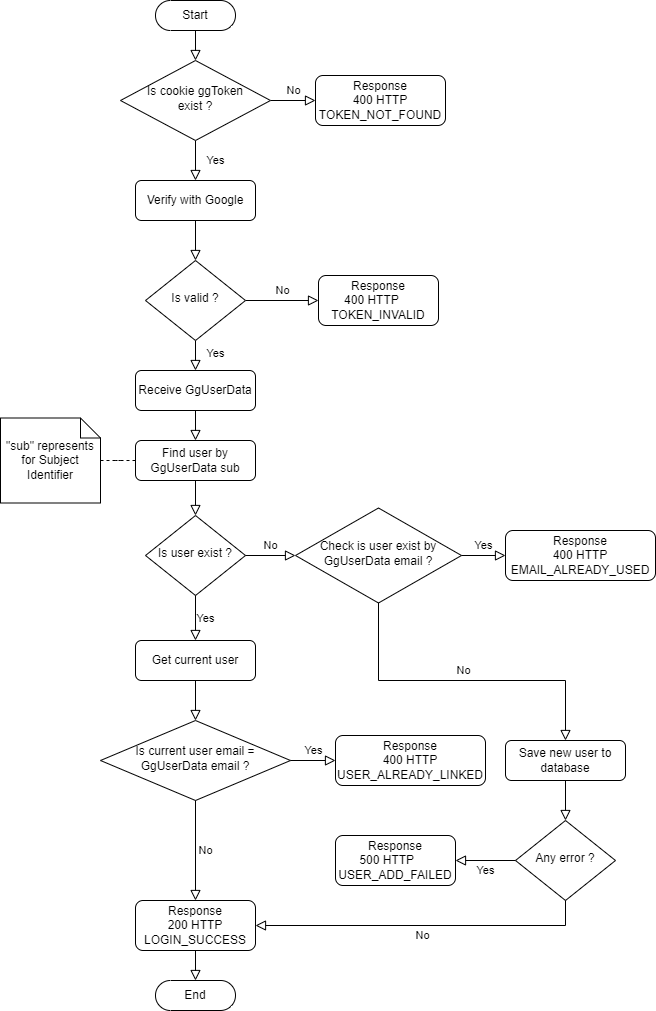
\includegraphics[width=\textwidth]{applied-thesis-chapters/chapter-4/Sơ đồ quá trình đăng ký và đăng nhập.png}
  \caption{Sơ đồ quá trình đăng ký và đăng nhập}
  \label{fig:SignUpIn}
\end{figure}

Ở bước “Verify with Google“ trong hình \ref{fig:SignUpIn} Sơ đồ quá trình đăng ký và đăng nhập, ta thực hiện xác thực credential nhận được với Google qua Authentication service.
Ở bước cuối cùng “Response Login Success“ cũng trong hình \ref{fig:SignUpIn} sơ đồ luồng kiểm tra đăng nhập, ngoài việc thực hiện trả về các thông tin trong hình ta còn thực hiện ghi hai cookie là accessToken và refreshToken lên toàn domain của ứng dụng, bao gồm cả tên miền chính và tiên miền con. Hai token này là hai JWT được tạo qua phương thức signJwt() của Authentication service.

Trong việc ghi cookie lên toàn domain của ứng dụng, có một vấn đề đó là nếu đang trong phiên bản phát triển, khi ứng dụng web chạy trên localhost hay 127.0.0.1 thì không nên thêm thuộc tính domain, việc chỉ định thuộc tính domain trong trường hợp này sẽ gây ra lỗi khiến cho không ghi được cookie. Lỗi này nằm ở thiết kết của cookie của HTTP. Chi tiết như sau:

\textit{“Chỉ các máy chủ trong domain được chỉ định mới có thể đặt cookie cho domain và các domain phải có ít nhất hai hoặc ba dấu chấm để ngăn các miền có dạng: ".com", ".edu" và " va.us"…“} \cite{chap4bib4}

Để xử lý vấn đề này nhóm thực hiện như sau, ở phần scripts trong tệp package.json trong ứng dụng Node.js của hệ thống.
Nhóm cài đặt đặt biến môi trường NODE\_ENV là "production" ở lệnh start và NODE\_ENV là "development" ở lệnh dev.
Để việc đặt giá trị cho biến môi trường, để có thể tương thích trên mọi môi trường (hệ điều hành) chạy Node.js thì nhóm sử dụng gói cross-env để cài đặt, hỗ trợ thực hiện tác vụ này. Sau đó nhóm cài đặt phương thức isOnProduction() để kiểm tra giá trị biến môi trường xem ứng dụng backend đang chạy trong chế độ (mode) nào. Và trước khi tiến hành ghi cookie sẽ tiến hành kiểm tra xem ứng dụng backend đang ở mode nào, nếu đang trong development mode thì sẽ không chỉ định thuộc tính domain và ngược lại.

\subsubsection{Cài đặt chức  năng đăng xuất}

\tab Khi người dùng chọn đăng xuất thì ứng dụng web sẽ tiến hành làm mới dữ liệu trong auth store. Đồng thời xóa hai cookie accessToken và refreshToken đã ghi trước đó.

Khi đó biến isAuth trong auth store, được cài đặt là biến phụ thuộc (dependence) trên phạm vi toàn ứng dụng web, có giá trị thay đổi thành false. Điều này khởi chạy các logic điều hướng người dùng trong ứng dụng ra ngoài màn hình trang chủ.

\subsection{Cài đặt chức năng dùng thử quét với ZAP Spider} \label{subsec:CaiDatDungThuZapSpider}

\tab Ở ứng dụng web, nhóm tạo một query endpoint với RTK Query đặt tên là trialScan, endpoint thuộc loại Query endpoint, là một endpoint tùy chỉnh (custom endpoint) để có thể sử dụng SSE, streaming update, đã đề cập đến ở phần "Endpoints, Queries, Mutations, các lifecycle hook và Streaming Update" của mục \ref{sec:RTKQ}.
Endpoint nhận vào tham số target kiểu chuỗi (string) và trả về data custom được mô tả trong bảng \ref{tab:DesDataTrial}.

\begin{tabularx}{\textwidth}{|>{\hsize=.15\hsize\centering\let\newline
  \\\arraybackslash}X|>{\hsize=.15\hsize\centering\let\newline
  \\\arraybackslash}X|>{\hsize=.60\hsize\raggedright\let\newline
  \\\arraybackslash}X|}
  \hline
  \thead{Tên              \\thuộc tính}
   & \thead{Kiểu dữ liệu}
   & \thead{Mô tả}
  \\
  \hline
  isScanning
   &
  boolean
   &
  Thuộc tính cho biết endpoint đang trong quá trình quét hay không
  \\
  \hline
  progress
   &
  number
   &
  Thuộc tính cho biết tiến triển phần trăm của quá trình quét
  \\
  \hline
  data
   &
  string[]
   &
  Thuộc tính lưu trữ các In Scope URL mà ZAP Spider quét được
  \\
  \hline
  error
   &
  Status
   &
  Thuộc tính lưu trữ trạng thái lỗi nếu có lỗi phát sinh trong quá trình quét
  \\
  \hline
  \caption{Mô tả các thuộc tính của đối tượng data custom trong trialScan endpoint}
  \label{tab:DesDataTrial}
\end{tabularx}

Để thể hiện quá trình quét đang được thực hiện, trong hook onQueryStarted của trialScan endpoint ta dùng updateCachedData để cập nhật isScanning thành true. Tiếp đến, ta tiến hành thiết lập kết nối SSE với ứng dụng hệ thống trong hook onCacheEntryAdded. Khi trialScan endpoint được gọi, quá trình xử lý ở hai phía như sau:

Phía ứng dụng web, ta thiết lập kết nối SSE tới backend bằng cách sử dụng đối tượng EventSource trong JavaScript.
Endpoint được sử dụng để kết nối là /scan/trial?url="URL", với URL là địa chỉ trang web cần quét.
Sau thiết lập thành công, ta tiếp tục tạo lắng nghe sự kiện trên ba kênh “id”, “status” và “error”.

\begin{itemize}
  \item Kênh “id” dùng để lắng nghe mã số định danh phiên quét (scan id) của phiên quét.
  Nếu sự kiện gửi đến không hợp lệ thì đóng kết nối SSE và cập nhật lại isScanning thành false.
  \item Kênh “status” dùng để lắng nghe trạng thái tiến độ (progress status) của phiên quét và cập nhật lên data.
  Mỗi khi progress được gửi đến, cập nhật progress lên data và thực hiện lần lượt hai việc.
  \begin{itemize}
    \item Thứ nhất là gọi yêu cầu lấy dữ liệu từ endpoint /scan/trial/results?id=scanId bằng phương thức fetch() và cập nhật dữ liệu nhận được lên data, với scanId là scan id lắng nghe được từ kênh “id” và dữ liệu nhận được là chuỗi các URL kết quả quét từ phiên ZAP Spider trong thời điểm đó.
    Kết quả được xử lý lại nhất quán, không trùng lặp.
    \item Thứ hai là kiểm tra điều kiện duy trì kết nối nếu giá trị status là 100 thì đóng kết nối và cập nhật lại isScanning thành false.
    \item Kênh “error“ dùng để lắng nghe các trạng thái lỗi được gửi đến.
  \end{itemize}
  Nếu có bất kỳ trạng thái nào được gửi đến thì cập nhật thông tin lên error trong đối tượng data custom, đóng kết nối SSE và cập nhật isScanning thành false.
\end{itemize}

Phía ứng dụng hệ thống, cài đặt chức năng quét này khác biệt so với các chức năng quét khác.
Ứng dụng hệ thống thực hiện kết nối SSE trước và kiểm tra sự hợp lệ của URL sau, nếu URL không hợp lệ thì gửi trạng thái INVAVLID\_URL lên kênh “error”.

Để kiểm tra sự hợp lệ của URL, ngoài các cài đặt kiểm tra bình thường nhóm có cài đặt phương thức isValidURL() với điều kiện đặc biệt là: Không được bao gồm chuỗi “localhost“ và “127.0.01“; URL phải có giao thức "http" hoặc "https", sử dụng gói validator.

Cuối cùng start phiên quét và thực hiện đăng ký kết nối của ứng dụng web cho satus monitor tương ứng bằng ZAP Monitor service.
Phiên quét được start với các cấu hình mặc định cài đặt sẵn cho chức năng dùng thử với ZAP Spider.
Các cấu hình được biểu diễn chi tiết trong bảng \ref{tab:ConfigSpiderDefault}.

\begin{tabularx}{\textwidth}{|>{\hsize=.45\hsize\centering\let\newline
  \\\arraybackslash}X|>{\hsize=.45\hsize\centering\let\newline
  \\\arraybackslash}X|}
  \hline
  \thead{Tên thuộc tính}
   & \thead{Cài đặt thuộc tính}
  \\
  \hline
  maxChildren
   &
  5
  \\
  \hline
  recurse
   &
  true
  \\
  \hline
  contextName
   &
  ""
  \\
  \hline
  subtreeOnly
   &
  false
  \\
  \hline
  \caption{Bảng chi tiết cấu hình mặc định cho chức năng dùng thử với ZAP Spider}
  \label{tab:ConfigSpiderDefault}
\end{tabularx}

\subsection{Cài đặt chức năng quản lý mục tiêu}

\tab Để hiển thị thông tin chi tiết các target ở ứng dụng web, nhóm cài đặt getTarget endpoint là một Query endpoint, endpoint thực hiện request HTTP GET đến điểm /management/targets để lấy danh sách thông tin các target. Để getTarget endpoint biết được khi nào data đã cũ thì nhóm cung cấp tag TARGET\_TAG cho hook providesTags.

Ở ứng dụng hệ thống, vì các endpoint trong chức năng quản lý mục tiêu là các endpoint cần xác minh người dùng nên sẽ được đặt dưới các middleware xác thực từ Authentication service. Danh sách thông tin được lấy thông qua target.model với định danh người dùng tương ứng, không bị đánh dấu xóa, sắp xếp theo thứ tự giảm dần ở thuộc tính updateAt và gửi đi.

\subsubsection{Cài đặt chức năng tạo và xóa mục tiêu}

\tab Để thêm mới target, ở ứng dụng web, nhóm cài đặt addTarget endpoint là một Mutation endpoint, endpoint thực hiện request HTTP POST đến /management/target.
Để đánh dấu danh sách target trong cache đã cũ sau khi thêm mới thì nhóm thêm tag TARGET\_TAG, giống với getTarget endpoint, cho hook invalidatesTags trong endpoint.
Ở ứng dụng hệ thống, thực hiện kiểm tra lại target với phương thức isValidURL() (đã nhắc đến ở mục \ref{subsec:CaiDatDungThuZapSpider}) và kiểm tra target có bị trùng tên với nhóm các target đã có của người dùng không. Nếu tất cả đều thỏa thì thêm target vào database. Endpoint gửi và nhận về kết quả trạng thái tương ứng trong bảng MGMT\_STATUS.

Để xóa target, ở dứng dụng web, nhóm cài đặt moveToTrashTarget endpoint loại Mutation endpoint, thực hiện request HTTP DELETE đến /management/target?id=”ID” với ID là id của target.

Để đánh dấu danh sách target trong cache đã cũ sau khi xóa thì nhóm thực hiện tương tự addTarget endpoint, thêm tag TARGET\_TAG vào hook invalidatesTags.

Ở ứng dụng hệ thống, thực hiện xóa target qua các bước: kiểm tra hợp lệ tham số trên query; kiểm tra sự tồn tại của target bằng target id và user id, nếu hợp lệ thì thực hiện cập nhật thuộc tính idDelete của target đó thành true.

\subsubsection{Cài đặt chức năng tìm mục tiêu theo tên}

\tab Để thực hiện chức năng này, nhóm chỉ thực hiện cài đặt ở phía ứng dụng web. Danh sách các target được nhóm phân biệt theo hai đối đượng. Một là đối tượng danh sách các target có từ endpoint gọi là listTarget, hai là danh sách các target dùng để hiển thị gọi là listShowTarget. listShowTarget là một đối tượng được phản chiếu từ listTarget, các thay đổi trên thanh tìm kiếm sẽ thực hiện lọc và thay đổi listShowTarget.

Khi thực hiện tác vụ trên, nhóm gặp vấn đề vì thông tin trong thanh tìm kiếm là thông tin được nhập từ người dùng, nên tác vụ lọc sẽ được thực hiện rất nhiều lần khi thông tin tìm kiếm thay đổi. Đều này gây ra vấn đề hiệu suất và hiển thị. Để giải quyết vấn đề trên nhóm cài đặt custom hook useDebounceEffect(), sử dụng kỹ thuật debounce, để kiểm soát tầng suất thực hiện tác vụ. Sau đó, nhóm thực hiện bao tác vụ tìm kiếm và lọc trong hook này để khi người dùng dừng thay đổi thông tin tìm kiểm trong một khoảng thời gian thì mới thực hiện lọc. Khoảng thời gian nhóm cài đặt là 300 mili giây.

\subsection{Cài đặt chức năng tạo phiên quét}

\tab Để có thể gửi yêu cầu quét của các loại quét cho ứng dụng hệ thống, ở ứng dụng web, nhóm cài đặt lần lượt các endpoint cho các loại quét với các tên spiderScan, ajaxScan, passiveScan, activeScan. Các endpoint này đều là Mutation endpoint thực hiện request HTTP POST đến lần lượt các điểm /scan/zap/spider, /scan/zap/ajax, /scan/zap/passive, /scan/zap/active. Các endpoint này đều gửi thông tin target cần quét, riêng passiveScan và activeScan thì cần thêm thông tin exploreType.

Để biết được target nào cần quét và sử dụng các loại quét nào, nhóm tạo một đối tượng danh sách các target được chọn trong store gọi là listSelectedTarget và một đối tượng lưu thông tin trạng thái các lựa chọn quét gọi là scanOption. Đối tượng listSelectedTarget là một mảng có các phần tử là đối tượng chứa một số thông tin của target, thông tin tiêu biểu là target id. Đối tượng scanOption là một đối tượng chứa thông tin trạng thái bật tắt của các loại quét. Cùng với đó, nhóm tạo các reducer tương ứng trong store để thực hiện thay đổi, thêm bớt cho các đối tượng này.

Ở giao diện web, theo cách tạo phiên quét bình thường, người dùng phải trải qua hai bước thiết lập là chọn các target trong danh sách và cấu hình các phiên quét.
Ở đây nhóm sẽ gọi đến các reducer tương ứng để lưu thông tin vào các đối tượng trong store. Cách tiếp cận này giúp nhóm có thể cài đặt hiển thị bền vững thông tin trạng thái của các lựa chọn trong màn hình, có nghĩa nếu đang trong quá trình tạo phiên quét, người dùng có di chuyển khỏi màn hình thì trạng thái của các lựa chọn cũng không mất đi.

Nhờ cách cài đặt này, người dùng có thể sử dụng chức năng này như chức năng tạo nhiều phiên quét cùng lúc.
Để bắt đầu xử lý gọi các phiên quét, nhóm tạo một custom hook tên useDigestTargetsWithOptions().
Hook sẽ được gọi khi người dùng chọn bắt đầu quét sau khi đã thực hiện lựa chọn xong.
Hook gọi đến lần lượt các trạng thái trong scanOption, ở mỗi trạng thái nếu là true thì sẽ duyệt listSelectedTarget và tạo phiên quét tương ứng với id target đó, gọi đến endpoint dùng để quét đã trình bày ở trên.
Sau khi hoàn thành mỗi lần start scan cho mỗi phiên quét, để làm mới lại danh sách phiên quét thì nhóm thực hiện đánh dấu cũ cho tag của endpoint lấy danh sách phiên quét (sẽ được trình bày trong mục \ref{subsec:CaiDatQuanLyPhienQuet}).
Sau khi hoàn thành thì hook gọi đến reducer tương ứng để làm mới listSelectedTarget và scanOption.

Ở ứng dụng hệ thống, vì các endpoint trong này cần xác minh nên sẽ được đặt dưới các middleware xác thực.
Đối với mỗi endpoint tương ứng sẽ thực hiện start các loại scan tương ứng thông qua ZAP Monitor service, ví dụ endpoint để start ajax sẽ gọi ajaxStartAndMonitor().
Quá trình thực hiện start scan tương tự nhau và được thể hiện qua các bước:

\begin{itemize}
  \item Bước 1: Xác minh sự tồn tại của target trong database thông qua target id. Nếu không target không tồn tại thì trả về đối tượng trạng thái TARGET\_FIND\_FAILED với HTTP\ 400.
  \item Bước 2: Lấy URL trong target ra và tiếp tục kiểm tra sự hợp lệ của URL. Nếu không hợp lệ thì trả về đối tượng trạng thái INVALID\_URL với HTTP\ 400.
  \item Bước 3: Tạo mới đối tượng scan session thông qua đối tượng scan-session.model. Với các dữ liệu là thông tin target, người dùng và cấu hình của phiên.
  \item Bước 4: Bắt đầu start và monitor phiên quét thông qua ZAP Monitor service. Ở đây ZAP Monitor service sẽ trả về một đối tượng định danh phiên quét, như đã nhắc ở phần "Cài đặt ZAP Client service" của mục \ref{subsec:CaiDatNhomZapService}.
  \item Bước 5: Kiểm tra đối tượng định danh phiên quét được trả về ở bước trên. Nếu đối tượng tồn tại thì tiếp tục. Nếu đối tượng không xác định nghĩa là phiên quét start không thành công. Khi đó thực hiện cập nhật trạng thái quét của scan session là FAILED và lưu đối tượng vào database. Bước tiếp theo trả về đối tượng trạng thái ZAP\_INITIALIZE\_FAIL với HTTP\ 500.
\end{itemize}

Ở ứng dụng web, khi thực hiện chức năng này, nhóm gặp khó khăn vì danh sách phiên quét sẽ hiển thị nhiều mục phiên quét.
Mà mỗi mục tùy theo loại phiên quét mà sử dụng endpoint khác nhau.
Nhưng không thể cài đặt theo cấu trúc điều kiện cho mỗi mục trong trường hợp này, vì endpoint là hook và React không cho phép sử dụng hook trong cấu trúc điều kiện.
Nhóm giải quyết vấn đề này bằng cách tạo từng component cho từng mục khác nhau, với mỗi mục thuộc mỗi loại phiên quét.
Trong component, thực hiện gọi hook endpoint kết nối SSE trên loại component tương ứng. 

\subsection{Cài đặt chức năng quản lý phiên quét} \label{subsec:CaiDatQuanLyPhienQuet}

\tab Để có được danh sách các phiên quét (scan session), ở ứng dụng web nhóm cài đặt getScanSession endpoint là một Query endpoint, endpoint thực hiện request HTTP GET đến điểm /management/scanSessions để lấy danh sách thông tin các scan session. Để getScanSession endpoint biết được khi nào data đã cũ thì nhóm cung cấp tag SCAN\_SESSION\_TAG cho hook providesTags trong endpoint.

Ở ứng dụng hệ thống, vì các endpoint cần xác minh nên được đặt dưới các middleware xác thực. Danh sách được lấy thông qua scan-session.model với định danh người dùng tương ứng, sắp xếp theo thứ tự giảm dần ở thuộc tính updateAt. Vì nhóm cần thêm thông tin của target kèm với thông tin của scan session tương ứng, nên nhóm sử dụng chức năng Population của mongoose (chức năng thay thế đại diện cho \$lookup aggregation của MongoDB). Khi cài đặt Schema cho scan-session.model, nhóm tạo tham chiếu đến id của document target, và khi truy xuất scan session nhóm sử dụng phương thức populate() để kèm theo thông tin của target tương ứng.

\subsubsection{Cài đặt chức năng xem trạng thái phiên quét}

\tab Để thể hiện thông tin trạng thái của một phiên quét trong danh sách quét, nhóm thiết lập hai loại thông tin là thông tin trạng thái (state) và thông tin trạng thái tiến triển (progess). State chỉ trạng thái hiện tại của phiên quét và được thể hiện trong dữ liệu của phiên quét đó. Có 3 loại state là PROCESSING, SUCCESSFUL và FAILED. Progress là thông chỉ tiến độ của phiên quét khi phiên quét đang trong state PROCESSING, vì vậy chỉ khi state của phiên quét là PROCESSING thì progress mới hiển thị. Tùy theo từng loại quét mà progress sẽ thể hiện khác nhau.

Để có được thông tin progress của phiên quét, ở ứng dụng web, nhóm cài đặt lần lượt các endpoint cho các loại phiên quét với các tên streamSpiderScan, streamAjaxScan, streamPassiveScan, streamActiveScan.
Các endpoint đều là Query endpoint và là custom endpoint để streaming update, đã đề cập đến ở phần "Endpoints, Queries, Mutations, các lifecycle hook và Streaming Update" của mục \ref{sec:RTKQ}.
Các endpoint này nhận vào tham số để định danh phiên quét tương ứng của nó ở ứng dụng hệ thống và trả về đối tượng data custom.
Đối tượng data custom có các thuộc tính tương như các thuộc tính được mô tả trong bảng "\ref{tab:DesDataTrial} Mô tả các thuộc tính của đối tượng data custom trong trialScan endpoint" của mục \ref{subsec:CaiDatDungThuZapSpider}.
Tuy nhiên, đối tượng không có thuộc tính data và thuộc tính progress sẽ có kiểu và giá trị tùy theo loại phiên quét. Nếu phiên quét thuộc loại ZAP Spider và ZAP Active thì thuộc tính progress sẽ là kiểu số và có giá trị từ 0 đến 100. Nếu phiên quét thuộc loại ZAP Ajax và ZAP Passive thì thuộc tính progress sẽ là kiểu chuỗi và có giá trị là “running“ hoặc “stopped“.

Các endpoint tiến hành thiết lập kết nối SSE với ứng dụng hệ thống trong hook onCacheEntryAdded bằng EventSource. Các endpoint được sử dụng để kết nối lần lượt tương ứng là \\
/scan/zap/spider?scanSession=”sessionId”\&zapScanId=”zapScanId”, \\
/scan/zap/ajax?scanSession=”sessionId”\&zapClientId=”zapClientId”, \\
/scan/zap/passive?scanSession=”sessionId”\&zapClientId=”zapClientId”, \\
active?scanSession=”sessionId”\&zapClientId=”zapClientId” với sessionId là định danh document của phiên quét, zapScanId và zapClientId chính là thông tin định danh của đối tượng đang thực hiện phiên quét.

Khi endpoint được gọi, endpoint cập nhật isScanning thành true trên hook onQueryStarted trước rồi thực hiện kết nối SSE với ứng dụng hệ thống trong hook onCacheEntryAdded.
Sau khi thiết lập thành công, tạo lắng nghe sự kiện trên hai kênh “status” và “error”.
\begin{itemize}
  \item Kênh “status” lắng nghe thông tin progress của phiên quét.
  Mỗi khi trạng thái được gửi đến, thực hiện cập nhật progress lên data và kiểm tra điều kiện duy trì kết nối nếu giá trị status là 100 hoặc “stopped“ thì đóng kết nối và cập nhật lại isScanning thành false.
  \item Kênh “error“ dùng để lắng nghe các trạng thái lỗi được gửi đến.
  Nếu trạng thái được gửi đến thì cập nhật thông tin lên error trong đối tượng data custom, đóng kết nối SSE và cập nhật isScanning thành false.
\end{itemize}

Phía ứng dụng hệ thống, quá trình thực hiện kết nối streamming update tương tự nhau trên các endpoint. Quá trình được thực hiện qua các bước:

\begin{itemize}
  \item Bước 1: Kiểm tra scanSession có tồn tại hợp lệ không và có thuộc về đúng user id không. Nếu không thì trả về đối tượng trạng thái INVALID\_SESSION với HTTP 400.
  \item Bước 2: Kiểm tra zapScanId hay zapClientId có tồn tại hợp lệ không. Nếu không thì trả về đối tượng trạng thái INVALID\_ID với HTTP 400.
  \item Bước 3: Thiết lập kết nối SSE.
  \item Bước 4: Lấy status monitor của phiên quét lên làm publisher qua ZAP Monitor service. Thực hiện kết nối publisher vào các kênh tương ứng ở SSE.
\end{itemize}

Ở ứng dụng web, khi thực hiện chức năng này, nhóm gặp khó khăn vì danh sách phiên quét sẽ hiển thị nhiều mục phiên quét và mỗi mục tùy theo loại phiên quét mà sử dụng endpoint khác nhau. Không cài đặt theo cấu trúc điều kiện cho mỗi mục trong trường hợp này, vì endpoint là hook và React không cho phép sử dụng hook trong cấu trúc điều kiện. Nhóm giải quyết vấn đề này bằng cách tạo từng component cho từng mục khác nhau, với mỗi mục thuộc mỗi loại phiên quét. Thực hiện gọi hook endpoint kết nối SSE trên loại component tương ứng.

\subsubsection{Cài đặt chức năng xem kết quả chi tiết phiên quét}

\tab Ở ứng dụng web, khi người dùng chọn vào một phiên quét trong danh sách quét được hiển thị, người dùng sẽ được đưa đến màn hình hiển thị thông tin chi tiết của phiên quét. Mỗi loại phiên quét khác nhau sẽ có cách hiển thị thông tin khác nhau. Xét chung, thông tin chi tiết phiên quét của các loại đều có hai phần là thông tin chi tiết của phiên quét (scan session) và thông tin chi tiết kết quả (full result).

Thông tin chi tiết của phiên quét được trích xuất từ data cache của endpoint getScanSession. Để tối ưu số lần gọi endpoint, nếu người dùng di chuyển vào màn hình khi data cache của endpoint getScanSession có tồn tại thì dữ liệu sẽ được trích xuất ở đó. Nếu data cache của endpoint getScanSession không tồn tại, ví dụ như trường hợp người dùng tải lại trang tại màn hình này, thì sẽ gọi đến endpoint.

Để có được thông tin chi tiết kết quả thì ta cần có id của chính phiên quét đó.
Id này sẽ được lấy từ scan session ở trên.
Để lấy full result, nhóm tạo các endpoint với các loại scan session tương ứng.
Các endpoint này đều là Query endpoint, endpoint thực hiện request HTTP GET đến các điểm \\
spider/fullResults?scanSession=${sessionId},\\
ajax/fullResults?scanSession=${sessionId},\\
passive/fullResults?scanSession=${sessionId},\\
active/fullResults?scanSession=${sessionId} với sessionId là scan session id ta có.
Tùy vào endpoint của từng loại quét mà kết quả sẽ khác nhau. Ở ứng dụng hệ thống, endpoint này của các loại quét được thiết kế xác thực, kiểm tra và truy vấn dữ liệu như thường.

Ở ứng dụng web, cách thể hiện giao diện màn hình của các loại quét cũng khác nhau.
Để thể hiện đầy đủ thông tin kết quả của phiên quét, nhóm thiết kế như sau.
Màn hình của mọi loại quét đều có hiển thị phần thông tin chi tiết của scan session, mục cấu hình sẽ khác nhau theo cấu trúc tương ứng loại quét, đã được mô tả ở phần "Cài đặt ZAP Client service" mục \ref{subsec:CaiDatNhomZapService}.

Phần tiếp theo trong màn hình là thông tin full result, để hiển thị full result của từng loại kết quả, nhóm phân giao diện phần này thành hai dạng chính. Một là dạng danh sách bảng các URL và hai là dạng chi tiết cảnh báo (alerts detail). Ở màn hình của phiên quét loại ZAP Spider và ZAP Ajax sẽ sử dụng các thành phần dạng danh sách bảng các URL. Và loại ZAP Passive và ZAP Active sẽ sử dụng các thành phần dạng alerts detail. Trong một alerts detail sẽ có 3 phần là tóm tắt cảnh báo (alerts summary), thông tin cảnh báo (alerts information) và chi tiết các cảnh báo (alerts detail).

Tương tự như phần "Cài đặt chức năng xem trạng thái phiên quét" mục \ref{subsec:CaiDatQuanLyPhienQuet}, vì React không cho phép sử dụng hook trong cấu trúc điều kiện. Nên nhóm phải cài đặt từng loại thành phần thông tin cho từng loại quét khác nhau. Và màn hình hiển thị thông tin chi tiết sẽ sử dụng các thành phần này tương ứng với nhu cầu.

\subsubsection{Cài đặt chức năng xuất tệp PDF kết quả chi tiết phiên quét}

\tab Khi đang trong màn hình hiển thị thông tin chi tiết của phiên quét, người dùng có thể xuất tệp PDF cho thông tin chi tiết này. Mỗi loại quét khác nhau sẽ có cấu trúc tệp PDF khác nhau. Tệp PDF này là phiên bản đầy đủ nhất, tham chiếu với dữ liệu của scan session và full result mà hệ thống lưu trữ.

Chức năng này được thực hiện bởi ứng dụng web. Để tương tác với tệp PDF bằng TypeScript, nhóm sử dụng gói jspdf là một thư viện mã nguồn mở được viết bằng JavaScript, cho phép tạo và xuất các tài liệu PDF trên trình duyệt web. Tuy nhiên, nhu cầu của nhóm đa phần là tạo bảng nhưng việc tạo bảng thông qua gói sẽ tạo ra rất nhiều công việc nằm ngoài phạm vi của khóa luận. Để có thể tạo bảng trong tệp PDF, nhóm đã tìm và sử dụng thêm gói jspdf-autotable là một phần mở rộng của gói jspdf. Gói jspdf-autotable có các tính năng hỗ trợ tạo bảng dữ liệu trong tài liệu PDF từ mảng dữ liệu, định dạng cột và hàng, tùy chỉnh chiều rộng của cột, chèn hình ảnh và các siêu liên kết vào bảng, và tạo các trang PDF có kích thước tùy chỉnh.

Tuy sự hỗ trợ mạnh mẽ từ gói, nhưng về bản chất đây là một tác vụ duyệt và ghi tệp PDF một cách thủ công.
Nên nhóm cần phải thực hiện một khối công việc nhất định cho chức năng này.
Tùy theo từng loại quét mà nội dung của tệp sẽ khác nhau.
Nhưng vẫn thứ tự xắp xếp và các dạng thông tin trong tệp được cấu trúc tương tự như đã nhắc ở phần "Cài đặt chức năng xem kết quả chi tiết phiên quét" của mục \ref{subsec:CaiDatQuanLyPhienQuet}.

Khi thực hiện chức năng này, nhóm gặp phải khó khăn đó là cộng đồng sử dụng tệp PDF trên ứng dụng web tuy lớn, nhưng phát triển không mạnh. Các công cụ hỗ trợ đa dạng nhưng chưa thực sự tốt và phù hợp với nhu cầu của chức năng. Tài liệu của các công cụ còn hạn chế. Để lựa chọn được gói phù hợp để thực hiện chức năng, nhóm thực hiện dùng thử hết các gói đến khi có gói phù hợp. Cuối cùng nhóm đúc kết được kết quả sử dụng kết hợp hai gói là jspdf và jspdf-autotable để thực hiện chức năng này.